%!TeX root = main.tex
\documentclass[main.tex]{subfiles}

\begin{document}

\chapter{Cation placement in zeolites}\label{cationzeolites}
\clearpage

Among the different families of adsorbents, zeolites are among the most used in industry. Small gases tend to adsorb preferentially on cations when they are present, which makes the study of cationic zeolites particularly relevant to the understanding of industrial adsorption processes. This chapter presents the chemical nature of cationic zeolites and explains the challenges and methods used to obtain representative models of them for subsequent adsorption simulations.% The central part of the chapter focuses on the newly developed ``shooting star'' methodology, which significantly reduces the amount of resource needed to compute the repartition of cations in zeolites.

\section{Cationic zeolites}

In this section, we detail the general structure of cationic zeolites and highlight the challenges associated with the simulation of such systems.

\subsection{Structure and properties}

Zeolites are a family of aluminosilicates, first discovered by Axel Fredrik Cronstedt in 1756. Similar to glass, their atomic structure is made of tetrahedra where the central atom, called a T-atom, is usually silicon, bridged together by oxygens. They are crystalline however, with typical unit cell lengths varying between \qty{10}{\angstrom} and \qty{100}{\angstrom}, and have nanopores.

The different kinds of zeolites are separated by topology: each known zeolite topology is given a capital three-letter code by the International Zeolite Association Structure Committee (IZA-SC). As explained in~\cref{topology_introduction}, the topology designates the information extracted from the network of chemical bonds: in the case of zeolites, this network can be simplified by taking one vertex per T-atom, and abstracting each oxygen bridge as a simple edge between the two corresponding T-atoms. The simplicity of this protocol makes it clear that the net of a zeolite is very close to the structure it represents --~in other words, simplifying the crystal into its net does not lose much information on the initial structure --~which explains why a classification by topology is the primary way to distinguish different zeolite structures. It is noteworthy that such a classification is vastly insufficient in the case of MOFs, where the chemistry of metal nodes and the nature of the ligands is thus used first; while for other kinds of materials such as glasses, it is downright impossible to establish because of the absence of cell periodicity.

While millions of hypothetical zeolite topologies have been identified by numerical methods\autocite{Deem}, only 256 have been experimentally observed as of 2024 (plus 9 intergrowth families, which are not strictly crystalline). This discrepancy may stem from the metastability of zeolites, whose porosity make them thermodynamically less favourable than glass\autocite{ZeoliteStability}. On the other hand, new experimental zeolite topologies have been discovered each year in the last twenty years, which indicates that accessing new structures is also limited by the current synthetic methods used. Moreover, new synthetic routes can allow new chemistry on existing topologies\autocite{ZeoliteSynthesisReviewJihong,ZeoliteSynthesisUnconventionalDusselier}.

Indeed, each given topology may give rise to several zeolites that differ by their exact chemical composition. Isoelectronic metal substitution consists in the replacement of silicon by germanium\autocite{GermaniumZeolites} or tin\autocite{TinZeolites}. A very common kind of substitution consists in replacing some T-atoms by aluminium, or, more anecdotally, boron\autocite{BoronZeolites} or gallium\autocite{GalliumZeolites}: each such substitution introduces one extra electron in the system, hence these zeolites contain cations to maintain electroneutrality. The nature of the cation itself leads to some more variability: sodium cations are usually the ones used during synthesis, and can then be exchanged with other cations\autocite{CationExchangeZeolites,CationsFAUReview}. Some other substitutions include transition metals such as titanium, iron or vanadium\autocite{ExoticZeoliteComposition,TinZeolites}. For simplicity, all zeolites discussed henceforth will be considered having only either Si or Al as T-atoms.

Ion exchange is currently the most prevalent industrial use case for cationic zeolites, especially as water softener for laundry agents\autocite{ZeoliteSynthesisUnconventionalDusselier}. Their considerable internal surface and the accessibility of active sites such as the cations or the substituted metals make them also useful for catalysis\autocite{ExoticZeoliteComposition}. Other applications include nuclear waste storage\autocite{ZeoliteRadioactive}, building material additives\autocite{ZeoliteConcrete}, water absorbents\autocite{ZeoliteWater}, soil treatment\autocite{ZeoliteSoil}, oxygen and contrast agent carrier for cancer treatment\autocite{ZeoliteCancer} and others. Finally, they can be used as adsorbents for gas separation or storage, which is also of capital industrial interest.

Zeolite structures are mostly considered rigid structures in simulations, although some notable exceptions exist\autocite{RHOFlexibility,MFIFlexibility}, and most actually posess a flexibility window\autocite{ZeoliteFlexibility} which is exploited, especially during adsorption\autocite{ZeoliteInducedFlexibility}. In addition, T-atom substitution tends to modify only slightly the T-O bond length (on average, Si-O: \qty{1.603}{\angstrom} while Al-O: \qty{1.736}{\angstrom}) and does not affect the O-T-O angles much, averaging at \qty{109.5}{\degree}\autocite{ZeoliteBondAngles}. As a consequence, the structure of a substituted zeolite can usually be well approximated by taking the reference structure of the topology (provided as a pure silicate by the IZA-SC) and replacing the relevant silicon atoms. However, not all placements of the substituents may correspond to existing zeolites

\subsection{Aluminium placement}

Cationic zeolites have some aluminiums as part of their structure, however their repartition among the T-atoms raises many questions.

\subsubsection{Rules}

The first rule, which is obeyed by almost all known zeolites, was discovered by Walter L\"owenstein \cite{Loewenstein}. It states that no two aluminiums may be neighbours, in the topological sense of being bridged by an oxygen. This hard rule limits the maximum number of aluminiums to half the number of T-atoms in general, and less for topologies that contain odd cycles: for instance, if there is a cycle of 5 T-atoms, only two among them can be aluminiums.

The amount of aluminiums in a zeolite is usually discussed in terms of \SiAl ratio. L\"owenstein's rule thus limits the minimal \SiAl ratio to 1, which corresponds to the maximum number of aluminiums and thus of cations. Zeolites with high \SiAl ratios, usually called high-silica zeolites, contain few cations and tend to be hydrophobic; they also tend to adsorb fewer molecules per unit cell since cations are privileged adsorption sites.

While L\"owenstein's rule is widely accepted as an axiom, and is mainly sustained by the absence of experimental synthesis of any zeolite with \SiAl ratio lower than 1, it is not currently proven. This comes from the cost of the few spectroscopic methods that allow identifying the precise locations of Al atoms: \ce{^{27}Al} and \ce{^{29}Si} magic-angle spinning NMR can be used to provide some limited information\autocite{ZeolitesMagicAngle}, while D{\v{e}}de{\v{c}}ek et al.\,\cite{ZeolitesAlPairs,ZeolitesAlPairs2} used UV-Visible-NIR spectroscopy on \ce{Co^{2+}}-exchanged ZSM-5 with high \SiAl ratio to retrieve their Al distribution. Yet, this method cannot be generalized to low-silica zeolites. Density Functional Theory (DFT) computation confirms the rule in general, but also shows potential violations for some zeolite topologies such as HEU\autocite{HEUnonLowenstein}.

The second rule, proposed by \textcite{Dempsey} on the basis of FAU zeolites with varying \SiAl ratios, states that when possible, the number of next-neighbours Al atoms should be minimized to decrease the number of unfavourable interactions between close aluminiums. This rule is actually known to be violated in many real zeolites, including dealuminated FAU. Speculatively, this may come from the fact that \textcite{Dempsey} made their observations on zeolites whose synthesis lead them to reach their global energy minimum, while many other synthetic routes can create structures trapped in a local energy minimum with respect to their \SiAl ordering.

\subsubsection{Simulation methodologies}

Overall, the lack of experimental evidence attesting to the precise position of aluminiums in zeolites make the theoretical prediction of such placement delicate, since it lacks verifiable comparison points. In particular, a crucial question is whether \SiAl ordering is truly guided by thermodynamical consideration or not\autocite{AlDistributionThermodynamic}. The latter case would appear for zeolites whose structure is in a metastable state, which is likely to be the case for many real zeolites as evidenced by \textcite{ZeolitesAlPairs2} in one of the few experimental studies tackling that very issue.

Even if the aluminium placement can be obtained as that which minimizes the global energy of the structure, this does not necessarily mean that the placement itself is periodic, nor that it should follow the same periodicity as the unit cell. Yet, as it is difficult to provide a concrete result on the localization of aluminiums without making such hypotheses, the studies in the literature only focus on the study of the placement of aluminiums in a single unit cell, supposing that the rest is periodic.

In these conditions, the last remaining question is the simulation methodology to use to find the global energy minimum of the structure. The most basic method consists in generating all possible configurations, computing their energy, and choosing that which minimizes the energy. This approach has actually been widely followed to find the preferred location of aluminiums when there are only one or two aluminiums per unit cell, using DFT to compute the energy\autocite{AlDistributionThermodynamic,AlDistributionFAUDFT}. The involved computational cost makes it impractical for lower \SiAl ratios however, which are of major interest for adsorption purposes.

Marie Jeffroy \cite{Jeffroy}\label{mariejeffroy_al} proposed a more refined Monte Carlo (MC) protocol for this problem, based on classical force fields for energy computation. Starting from a configuration with the target \SiAl ratio under L\"owenstein's rule, each MC step consists in exchanging the positions of a Si and an Al while maintaining L\"owenstein's rule, and accepting or rejecting the step according to the Metropolis-Hastings criterion (explained in \cref{metropolis}). For low \SiAl ratios, this algorithm requires adding some kind of ``restart'' option that entirely repopulates the aluminiums at random under L\"owenstein's rule, because that very rule can lead to blocked situation where no single \SiAl exchange is possible, as illustrated on \cref{fig:blocked_situation}.

\begin{figure}
	\centering
	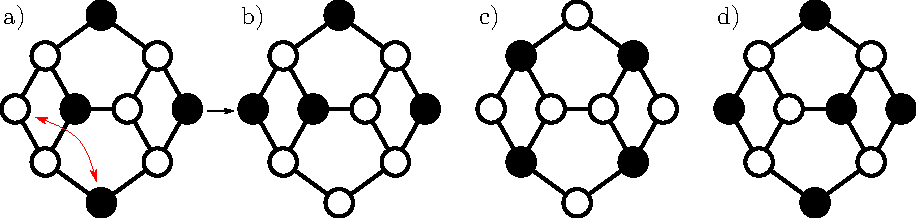
\includegraphics[width=\columnwidth]{figures/cations/blocked_situation.pdf}
	\caption{Schematic representation of aluminium placement in a zeolite fragment. Empty circles represent silicon, filled circles represent aluminium. Black edges represent -O- bridges. L\"owenstein's rule forbids two aluminiums from being neighbors.\\a) An exchange move between a silicon and an aluminium, used in Marie Jeffroy's scheme\autocite{Jeffroy}\\b) The result of the exchange\\c) A blocked configuration where no move is possible\\d) A configuration with one more aluminium, which cannot be reached from c)}\label{fig:blocked_situation}
\end{figure}

\Textcite{AlDistributionAlcanes} proposed an innovative method to assess the validity of theoretically-obtained aluminium placements, by studying alkane adsorption isotherms (defined in \cref{isotherms}). They found that different \SiAl orderings can lead to different isotherms, which, conversely, means that obtaining a precise experimental isotherm can allow retrieving the aluminium ordering. Their further study \cite{AlDistributionAlcanes2} determined that topologies LTL, FER, TON, and MOR exhibited isotherms sensitive to the aluminium placement, which could thus be retrieved from experimental adsorption isotherms, while FAU, LTA, MEL, and MFI were not sensitive enough. \Textcite{AlDistributionCO2Adsorption} reused a similar method with \ce{CO_2} isotherms instead, combined with reverse Monte Carlo method to tackle lower \SiAl ratios: they conclude that topologies LTA, CHA are more likely to have their aluminiums placed at random compared to FER.

Hence, given the uncertainty that any aluminium placements obtained by thermodynamical simulation actually reflects those observed in real zeolites, I chose to consider that the aluminium placement in our zeolites is taken at random. In practice, each zeolite with a given \SiAl ratio is modeled as the average of six zeolites of that topology with the same \SiAl ratio, all following L\"owenstein's rule but having different Al repartitions (taking symmetry into account as well). The results are computed on each of these six models, and averaged to obtain the result for the zeolite.

To obtain the zeolite structures with random aluminium placements obeying L\"owenstein's rule and the target \SiAl ratio, I implemented the following algorithm:
\begin{itemize}
    \item The starting point is either the zeolite filled with Si if the required \SiAl ratio is above 3, else a zeolite filled with as many Al as possible using a greedy algorithm. That greedy technique consists in doing a graph traversal of the T-atoms, transforming each atom into an Al if it is not the neighbour of an Al, or making it a Si otherwise: if all cycles in the graph are even, this is guaranteed to provide an aluminium placement with the minimal \SiAl of 1.
    \item The main algorithm then alternates between adjusting the number of Al and changing their positions, for a few steps each, back and forth.
    \begin{itemize}
        \item The position update follows the principle of Marie Jeffroy's MC scheme but disregarding the energy change: one Si is chosen at random among those that have no Al neighbor, then one Al is picked at random, and both are exchanged. This guarantees that the resulting structure still follows L\"owenstein's rule. No position update can occur if all Si have at least one Al neighbor.
        \item The number of Al atoms is modified if the current \SiAl ratio does not correspond to the target: if it is too high, an Al is converted into a Si, and otherwise a Si that has no Al neighbour is converted into an Al.
    \end{itemize}
    \item Since the situation can be blocked (see \cref{fig:blocked_situation}), the algorithm sometimes restart from scratch, or sometimes does a partial restart by converting multiple Al atoms into Si.
    \item Configurations with the closest \SiAl ratio to the target are kept in a set. Each configuration is assigned a hash, which is simply a sequence of 0 if the T-atom is a Si or 1 otherwise, in a fixed order of the T-atom. To avoid considering symmetry-equivalent configurations as different, the signature of a configuration is computed as the lexicographically minimum of all such hashes corresponding to the application of a symmetry operation on the configuration. For each unique signature, a corresponding unique configuration is then retained, and the six models are taken at random among these unique configurations.
\end{itemize}\label{aluminiumhash}

One last consideration is the choice of the supercell. It appears that, for a large number of zeolites topologies, the smallest unit cell cannot be filled with aluminiums so that it both obeys L\"owenstein's rule and reaches the minimal \SiAl ratio for that topology. In the case of LTA for instance, the smallest compatible cell is a $2\times2\times2$ supercell of the smallest unit cell. As a consequence, the greedy algorithm used before is launched on several supercells in an initial pass, and the one leading to the smallest \SiAl ratio is retained. This supercell is then used for all aluminium placement attempts on the same topology.

The full list of minimum \SiAl ratio found for each zeolite topology (except interrupted ones) and the respective supercell is presented in \cref{table:zeosial}. The supercell is considered with respect to the idealized framework available for each topology on the IZA-SC database\footnote{accessible at \url{https://europe.iza-structure.org/IZA-SC/ftc_table.php}}. This table presents the lowest \SiAl ratio found, but apart for the cases where it is $1$, the values here are not proven to be minimal, since the algorithm relies on random attempts. Similarly, the supercell used could be not minimal.

It is worth mentioning that a previous study of adsorption in zeolite by \textcite{WrongLowestSiAl1} claimed to use the lowest possible \SiAl ratios to screen through zeolites, but failed to reach the ones presented here, systematically in the case where a supercell needed to be used. Another by Daou, Fang, et al. \cite{WrongLowestSiAl2,WrongLowestSiAl3} alluded to that issue in the case of LTA, yet failed to identify some other topologies (ATT, JBY, LEV, LTL, MRT, OFF) which could reach an \SiAl ratio of 1. The choice of the supercell during aluminium placement is thus an easily overlooked, yet critical, point to consider.


\begin{table}
\small
\makebox[\textwidth]{%
\hspace{6pt}\begin{minipage}[t]{0.24\linewidth}
	\vspace{0pt}
	\begin{tabular}{|@{\hspace{0pt}}c@{\hspace{0pt}}|@{\hspace{1pt}}c@{\hspace{1pt}}|@{\hspace{2pt}}c@{\hspace{2pt}}|}
		\hline
		\scriptsize \bf Topology&\scriptsize \bf Si/Al&\scriptsize \bf Supercell\\\hline
ABW&$1$&1$\times$1$\times$1\\\hline
ACO&$1$&1$\times$1$\times$1\\\hline
AEI&$1$&1$\times$1$\times$1\\\hline
AEL&$1$&1$\times$1$\times$1\\\hline
AEN&$1$&1$\times$1$\times$1\\\hline
AET&$1$&1$\times$1$\times$1\\\hline
AFG&$1$&1$\times$1$\times$1\\\hline
AFI&$1$&1$\times$1$\times$1\\\hline
AFN&$1$&1$\times$1$\times$1\\\hline
AFO&$1$&1$\times$1$\times$1\\\hline
AFR&$1$&2$\times$2$\times$4\\\hline
AFS&$1$&1$\times$1$\times$1\\\hline
AFT&$1$&1$\times$1$\times$1\\\hline
AFV&$1$&3$\times$3$\times$2\\\hline
AFX&$1$&1$\times$1$\times$1\\\hline
AFY&$1$&1$\times$1$\times$1\\\hline
AHT&$1$&1$\times$1$\times$1\\\hline
ANA&$1$&1$\times$1$\times$1\\\hline
ANO&$1$&1$\times$1$\times$1\\\hline
APC&$1$&1$\times$1$\times$1\\\hline
APD&$1$&1$\times$1$\times$1\\\hline
AST&$1$&1$\times$1$\times$1\\\hline
ASV&$1$&1$\times$1$\times$1\\\hline
ATN&$1$&1$\times$1$\times$1\\\hline
ATO&$1$&1$\times$1$\times$1\\\hline
ATS&$1$&1$\times$1$\times$1\\\hline
ATT&$1$&3$\times$4$\times$3\\\hline
ATV&$1$&1$\times$1$\times$1\\\hline
AVE&$1$&1$\times$1$\times$1\\\hline
AVL&$1$&3$\times$3$\times$2\\\hline
AWO&$1$&1$\times$1$\times$1\\\hline
AWW&$1$&2$\times$2$\times$4\\\hline
BCT&$1$&1$\times$1$\times$1\\\hline
BEC&$1.29$&2$\times$2$\times$2\\\hline
BIK&$1.4$&4$\times$2$\times$5\\\hline
BOF&$1.4$&2$\times$1$\times$1\\\hline
BOG&$1.4$&1$\times$1$\times$1\\\hline
BOZ&$1.88$&1$\times$1$\times$1\\\hline
BPH&$1$&1$\times$1$\times$1\\\hline
BRE&$1.29$&4$\times$2$\times$4\\\hline
BSV&$1$&1$\times$1$\times$1\\\hline
CAN&$1$&1$\times$1$\times$1\\\hline
CAS&$1.4$&1$\times$1$\times$1\\\hline
CDO&$1.62$&4$\times$2$\times$2\\\hline
CFI&$1.46$&2$\times$5$\times$1\\\hline
CGF&$1$&2$\times$2$\times$4\\\hline
CGS&$1$&1$\times$1$\times$1\\
\end{tabular}
\end{minipage}\hspace{4pt}
\begin{minipage}[t]{0.24\linewidth}
	\vspace{0pt}
	\begin{tabular}{|@{\hspace{2pt}}c@{\hspace{2pt}}|@{\hspace{2pt}}c@{\hspace{2pt}}|@{\hspace{2pt}}c@{\hspace{2pt}}|}
CHA&$1$&1$\times$1$\times$1\\\hline
CON&$1.33$&1$\times$1$\times$1\\\hline
CSV&$1.22$&1$\times$2$\times$1\\\hline
CZP&$1$&1$\times$1$\times$1\\\hline
DAC&$1.57$&1$\times$3$\times$2\\\hline
DDR&$1.73$&1$\times$2$\times$1\\\hline
DFO&$1$&2$\times$2$\times$2\\\hline
DFT&$1$&4$\times$4$\times$3\\\hline
DOH&$1.62$&1$\times$2$\times$1\\\hline
DON&$1.29$&1$\times$1$\times$1\\\hline
EAB&$1$&1$\times$1$\times$1\\\hline
EDI&$1$&4$\times$4$\times$4\\\hline
EEI&$1.44$&1$\times$1$\times$1\\\hline
EMT&$1$&1$\times$1$\times$1\\\hline
EON&$1.4$&2$\times$1$\times$1\\\hline
EOS&$1.18$&1$\times$2$\times$2\\\hline
EPI&$1.74$&4$\times$2$\times$3\\\hline
ERI&$1$&1$\times$1$\times$1\\\hline
ESV&$1.4$&1$\times$1$\times$1\\\hline
ETL&$1.48$&2$\times$1$\times$1\\\hline
ETR&$1$&1$\times$1$\times$1\\\hline
ETV&$1.33$&1$\times$1$\times$1\\\hline
EUO&$1.49$&1$\times$1$\times$1\\\hline
EWF&$1.49$&2$\times$1$\times$1\\\hline
EWO&$1.4$&2$\times$2$\times$5\\\hline
EWS&$1.53$&1$\times$1$\times$1\\\hline
EZT&$1$&1$\times$1$\times$1\\\hline
FAR&$1$&1$\times$1$\times$1\\\hline
FAU&$1$&1$\times$1$\times$1\\\hline
FER&$1.57$&1$\times$1$\times$3\\\hline
FRA&$1$&1$\times$1$\times$1\\\hline
GIS&$1$&1$\times$1$\times$1\\\hline
GIU&$1$&1$\times$1$\times$1\\\hline
GME&$1$&1$\times$1$\times$1\\\hline
GON&$1.29$&1$\times$1$\times$1\\\hline
GOO&$1$&1$\times$1$\times$1\\\hline
HEU&$1.25$&1$\times$1$\times$2\\\hline
IFO&$1$&1$\times$1$\times$1\\\hline
IFR&$1.29$&1$\times$1$\times$2\\\hline
IFW&$1.29$&1$\times$1$\times$1\\\hline
IFY&$1$&1$\times$1$\times$2\\\hline
IHW&$1.55$&1$\times$1$\times$1\\\hline
IMF&$1.55$&1$\times$1$\times$1\\\hline
IRN&$1.19$&1$\times$1$\times$1\\\hline
IRR&$1.6$&2$\times$2$\times$2\\\hline
ISV&$1.31$&2$\times$2$\times$1\\\hline
ITE&$1.56$&1$\times$2$\times$1\\\hline
ITG&$1.33$&1$\times$1$\times$2\\
\end{tabular}
\end{minipage}\hspace{0pt}
\begin{minipage}[t]{0.24\linewidth}
\vspace{0pt}
\begin{tabular}{|@{\hspace{2pt}}c@{\hspace{2pt}}|@{\hspace{2pt}}c@{\hspace{2pt}}|@{\hspace{2pt}}c@{\hspace{2pt}}|}
ITH&$1.33$&1$\times$2$\times$1\\\hline
ITR&$1.33$&1$\times$1$\times$1\\\hline
ITT&$1.56$&2$\times$2$\times$3\\\hline
ITW&$1.4$&1$\times$1$\times$1\\\hline
IWR&$1.33$&2$\times$2$\times$2\\\hline
IWS&$1.27$&1$\times$1$\times$2\\\hline
IWV&$1.62$&1$\times$1$\times$2\\\hline
IWW&$1.33$&1$\times$1$\times$1\\\hline
JBW&$1$&5$\times$4$\times$3\\\hline
JNT&$1$&1$\times$1$\times$1\\\hline
JOZ&$1.5$&2$\times$1$\times$1\\\hline
JRY&$1$&1$\times$1$\times$1\\\hline
JSN&$1$&3$\times$4$\times$2\\\hline
JSR&$1.67$&1$\times$1$\times$1\\\hline
JST&$2$&1$\times$1$\times$1\\\hline
JSW&$1$&1$\times$1$\times$1\\\hline
JSY&$1$&1$\times$1$\times$1\\\hline
JZO&$1.37$&1$\times$1$\times$1\\\hline
JZT&$1.35$&1$\times$1$\times$1\\\hline
KFI&$1$&1$\times$1$\times$1\\\hline
LAU&$1$&2$\times$2$\times$4\\\hline
LEV&$1$&3$\times$3$\times$2\\\hline
LIO&$1$&1$\times$1$\times$1\\\hline
LOS&$1$&1$\times$1$\times$1\\\hline
LOV&$1.25$&2$\times$2$\times$1\\\hline
LTA&$1$&2$\times$2$\times$2\\\hline
LTF&$1.27$&1$\times$1$\times$4\\\hline
LTJ&$1$&1$\times$1$\times$1\\\hline
LTL&$1$&2$\times$2$\times$4\\\hline
LTN&$1$&1$\times$1$\times$1\\\hline
MAR&$1$&1$\times$1$\times$1\\\hline
MAZ&$1.4$&1$\times$1$\times$2\\\hline
MEI&$1.43$&1$\times$1$\times$1\\\hline
MEL&$1.67$&1$\times$1$\times$1\\\hline
MEP&$1.71$&1$\times$1$\times$1\\\hline
MER&$1$&1$\times$1$\times$1\\\hline
MFI&$1.67$&1$\times$1$\times$1\\\hline
MFS&$1.45$&3$\times$1$\times$1\\\hline
MON&$1.67$&2$\times$2$\times$1\\\hline
MOR&$1.67$&1$\times$1$\times$2\\\hline
MOZ&$1$&1$\times$1$\times$4\\\hline
MRT&$1$&2$\times$4$\times$2\\\hline
MSE&$1.55$&1$\times$1$\times$1\\\hline
MSO&$1$&2$\times$2$\times$2\\\hline
MTF&$1.44$&1$\times$1$\times$2\\\hline
MTN&$1.72$&1$\times$1$\times$1\\\hline
MTT&$1.4$&1$\times$1$\times$1\\\hline
MTW&$1.33$&1$\times$5$\times$3\\
\end{tabular}
\end{minipage}\hspace{2pt}
\begin{minipage}[t]{0.24\linewidth}
\vspace{0pt}
\begin{tabular}{|@{\hspace{2pt}}c@{\hspace{2pt}}|@{\hspace{2pt}}c@{\hspace{2pt}}|@{\hspace{2pt}}c@{\hspace{2pt}}|}
MVY&$1$&1$\times$1$\times$1\\\hline
MWF&$1$&1$\times$1$\times$1\\\hline
MWW&$1.53$&2$\times$2$\times$1\\\hline
NAB&$1.5$&2$\times$2$\times$1\\\hline
NAT&$1.22$&2$\times$2$\times$4\\\hline
NES&$1.52$&1$\times$1$\times$1\\\hline
NON&$1.44$&1$\times$1$\times$1\\\hline
NPO&$2$&4$\times$4$\times$5\\\hline
NPT&$2$&2$\times$2$\times$2\\\hline
NSI&$1.4$&2$\times$5$\times$3\\\hline
OBW&$1.92$&1$\times$1$\times$1\\\hline
OFF&$1$&3$\times$3$\times$4\\\hline
OKO&$1.62$&1$\times$1$\times$1\\\hline
OSI&$1$&1$\times$1$\times$1\\\hline
OSO&$2$&1$\times$1$\times$1\\\hline
OWE&$1$&2$\times$4$\times$3\\\hline
PAU&$1$&1$\times$1$\times$1\\\hline
PCR&$1.5$&1$\times$1$\times$1\\\hline
PHI&$1$&1$\times$1$\times$1\\\hline
PON&$1$&1$\times$1$\times$1\\\hline
POR&$1$&1$\times$1$\times$1\\\hline
POS&$1.29$&1$\times$1$\times$1\\\hline
PSI&$1$&1$\times$1$\times$1\\\hline
PTF&$1.5$&1$\times$1$\times$1\\\hline
PTO&$1.4$&1$\times$1$\times$1\\\hline
PTT&$1$&1$\times$1$\times$1\\\hline
PTY&$1.5$&1$\times$1$\times$1\\\hline
PUN&$1.25$&1$\times$1$\times$1\\\hline
PWN&$1$&1$\times$1$\times$1\\\hline
PWO&$1.5$&1$\times$1$\times$1\\\hline
PWW&$1.5$&1$\times$1$\times$1\\\hline
RFE&$1.4$&1$\times$1$\times$1\\\hline
RHO&$1$&1$\times$1$\times$1\\\hline
RRO&$1.25$&2$\times$1$\times$1\\\hline
RSN&$1.59$&4$\times$1$\times$4\\\hline
RTE&$1.4$&1$\times$1$\times$2\\\hline
RTH&$1.53$&2$\times$1$\times$3\\\hline
RUT&$1.57$&2$\times$2$\times$3\\\hline
RWR&$1.6$&4$\times$4$\times$1\\\hline
RWY&$3$&1$\times$1$\times$1\\\hline
SAF&$1$&1$\times$1$\times$1\\\hline
SAO&$1$&1$\times$1$\times$1\\\hline
SAS&$1$&1$\times$1$\times$1\\\hline
SAT&$1$&1$\times$1$\times$1\\\hline
SAV&$1$&1$\times$1$\times$1\\\hline
SBE&$1$&1$\times$1$\times$1\\\hline
SBN&$1.5$&1$\times$2$\times$1\\\hline
SBS&$1$&1$\times$1$\times$1\\
\end{tabular}
\end{minipage}\hspace{7pt}
\begin{minipage}[t]{0.24\linewidth}
\vspace{0pt}
\begin{tabular}{|@{\hspace{2pt}}c@{\hspace{2pt}}|@{\hspace{2pt}}c@{\hspace{2pt}}|@{\hspace{2pt}}c@{\hspace{2pt}}|}
SBT&$1$&1$\times$1$\times$1\\\hline
SEW&$1.36$&1$\times$2$\times$1\\\hline
SFE&$1.33$&1$\times$1$\times$1\\\hline
SFF&$1.46$&2$\times$1$\times$2\\\hline
SFG&$1.47$&1$\times$2$\times$2\\\hline
SFH&$1.29$&5$\times$1$\times$2\\\hline
SFN&$1.29$&1$\times$5$\times$2\\\hline
SFO&$1$&2$\times$2$\times$4\\\hline
SFS&$1.67$&1$\times$1$\times$1\\\hline
SFW&$1$&1$\times$1$\times$1\\\hline
SGT&$1.49$&2$\times$2$\times$1\\\hline
SIV&$1$&1$\times$1$\times$1\\\hline
SOD&$1$&1$\times$1$\times$1\\\hline
SOF&$1.5$&1$\times$1$\times$1\\\hline
SOR&$1.18$&1$\times$1$\times$2\\\hline
SOS&$1.4$&2$\times$4$\times$3\\\hline
SOV&$1.29$&1$\times$1$\times$1\\\hline
SSF&$1.25$&2$\times$2$\times$2\\\hline
SSY&$1.33$&1$\times$1$\times$1\\\hline
STF&$1.46$&1$\times$1$\times$2\\\hline
STI&$1.25$&1$\times$1$\times$1\\\hline
STT&$1.46$&1$\times$1$\times$1\\\hline
STW&$1.5$&1$\times$1$\times$1\\\hline
SVV&$1.33$&1$\times$1$\times$1\\\hline
SWY&$1$&1$\times$1$\times$1\\\hline
SZR&$1.25$&1$\times$1$\times$2\\\hline
TER&$1.35$&1$\times$1$\times$1\\\hline
THO&$1$&2$\times$4$\times$4\\\hline
TOL&$1$&1$\times$1$\times$1\\\hline
TON&$1.4$&2$\times$2$\times$5\\\hline
TSC&$1$&1$\times$1$\times$1\\\hline
TUN&$1.53$&1$\times$1$\times$1\\\hline
UEI&$1$&1$\times$1$\times$1\\\hline
UFI&$1.29$&2$\times$2$\times$1\\\hline
UOS&$1.18$&2$\times$4$\times$3\\\hline
UOV&$1.38$&1$\times$1$\times$1\\\hline
UOZ&$1$&1$\times$1$\times$1\\\hline
USI&$1$&1$\times$1$\times$1\\\hline
UTL&$1.62$&1$\times$2$\times$2\\\hline
UWY&$1.37$&1$\times$2$\times$3\\\hline
VET&$1.43$&1$\times$1$\times$1\\\hline
VFI&$1$&1$\times$1$\times$1\\\hline
VNI&$1.73$&3$\times$3$\times$1\\\hline
VSV&$1.78$&4$\times$4$\times$1\\\hline
WEI&$1.5$&1$\times$1$\times$1\\\hline
YFI&$1.4$&1$\times$1$\times$1\\\hline
YUG&$1.56$&3$\times$2$\times$4\\\hline
ZON&$1$&4$\times$2$\times$2\\\hline
	\end{tabular}
\end{minipage}\hspace{-2em}
}
\normalsize
	\caption{Minimal Si/Al and corresponding supercell obtained for all 239 non-interrupted topologies}
	\label{table:zeosial}
%\end{minipage}
\end{table}

\subsection{Cations}

The electroneutrality of the framework requires that each negative charge introduced by an Al substitution be compensated by the introduction of a cation in the framework. In many cases, \ce{Na^+} or \ce{H^+} are used during synthesis; they are sometimes replaced by other cations in later steps.

These cations have a primordial role for adsorption processes, because they constitute privileged adsorption sites for many small gases. The precise mechanism by which they contribute to the overall adsorption capacity of a material depends on their nature, their location, and the nature of the guest molecule however. Moreover, in addition to simple one-to-one adsorption cases of a small molecule on a cation, X-ray spectroscopy evidences the presence of adsorption complexes involving several cations and guest molecules at the same time\autocite{MultipleCationsMultipleSites}. Finally, the very nature of the cations present in the structure can be quite diverse, ranging from monovalent alkali to polyvalent metal ions, and even molecular ions such as many of the organic structure directing agents (OSDAs) used during zeolite synthesis.

In order to perform numerical simulation of the adsorption process, it is thus necessary to have a model of the zeolite that places its cations in the correct positions. Fortunately, and opposite to the previous case of aluminiums, X-ray diffraction is a convenient technique which can be used to obtain the crystallographic sites in which the cations are located, as well as the respective occupancy of each such site.


\section{Methodology for the prediction of cation placement}

While experimental cation maps are available on some zeolite structures, two seminal problems remain. First, when screening through a large amount of zeolite topologies and \SiAl ratio, only a small fraction of structures have their experimental cation map available. Second, even with the crystallographic sites, not all cation repartitions that obey the given occupancies have the same energy. For example, the site I and I' of FAU being very close to one another, the occupation of a site I prevents either of the neighbouring sites I' from being occupied at the same time. Deciding on the exact location of cations in a zeolite model is thus no trivial matter.

\subsection{Underlying algorithms}

To obtain equilibrium data, such as average positions, on molecular systems, there are two general simulation frameworks which can be used: molecular dynamics and Monte Carlo simulation. I only used Monte Carlo and its variations because they are the only strategy available to study a variable number of molecules, which is necessary for the simulation of adsorption as we will explain in more details in \cref{GCMC}. The possible use of molecular dynamics and its variants will be discussed later in \cref{metadynamics}.

\subsubsection{Canonical Monte Carlo direct simulation}
% mention ergodicity

The Monte Carlo (MC) method designates a large variety of algorithms which all converge towards their result by performing multiple random samplings. A wide subset of these form the Markov Chain Monte Carlo (MCMC) schemes, which are a class of algorithms that aim at sampling a target probability distribution. In the context of statistical physics, such methods provide practical ways of obtaining macroscopic observable values from the simulation of the microscopic behaviour of particles. Indeed, an observable $\mathcal O$ can be computed as the ensemble average of its microscopic counterpart $\left<o\right>$, which can be obtained from an integral over the configuration space. For example, in the canonical ensemble where the number of particles, the external temperature $T$ and the volume of the system is fixed, \[\mathcal O = \left<o\right> = \frac1Z\int\!\text d{\boldsymbol p}\  o\left({\boldsymbol p}\right)\exp\left(-\beta U\left({\boldsymbol p}\right)\right)\label{eq:canonicalensemble}\] where $\beta = 1/k_BT$, $U\left({\boldsymbol p}\right)$ is the energy of configuration $\boldsymbol p$ and $Z$ is the partition function. In other words, $\mathcal O$ can be computed as an integral of values of $o$ on a probability distribution of $\boldsymbol p$ given by $\boldsymbol p\mapsto \frac1Z\exp\left(-\beta U\left({\boldsymbol p}\right)\right)$.

The direct evaluation of this probability distribution is impossible in general, because of the partition function $Z$ whose value cannot be computed. Instead, the MCMC method gives a way to directly evaluate the observable $\mathcal O$ by providing a sequence of configurations $\{\boldsymbol p\}$ that follows the same probability distribution as the target. The integral can then be computed as simply the average value of $o$ on this specific set of configurations $\{\boldsymbol p\}$.

\label{metropolis}

The Metropolis-Hastings algorithm is the most common MCMC scheme used to provide such a sequence of configurations. It consists in starting from an initial state, \textit{i.e.} an initial position for all the mobile particles of the system, and making it evolve through a sequence of steps. At each step, a trial move, \textit{i.e.}, a modification of the state, is attempted and may, or may not, be accepted with a certain probability. In the case of a simulation in the canonical ensemble, the difference of energy $\Delta E$ between after and before the move gives the probability
\[P_\text{accept}(\Delta E) = \min\left(1, \exp\left(-\beta \Delta E\right)\right)\label{eq:MCcanonicalaccept}\]
that the move be accepted. Intuitively, this means that any move that decreases the energy of the system is accepted, while the others are accepted with a probability that decreases as the energy difference increases, sharply at low temperature and more slowly at high temperature. In the limit of infinite temperature, all the moves are accepted; at zero temperature, only the moves that decrease the energy are. The details on how to compute energy are deferred to \cref{energy_computation}.

To avoid drift, the algorithm obeys detailed balance which, conceptually, represents the microreversibility of the simulated physical processes. In practice, this means that, for each MC move that brings the system from configuration ${\boldsymbol p}_\mathcal{A}$ to ${\boldsymbol p}_\mathcal{B}$, there must exist a ``converse'' MC moves that can bring the system from $\mathcal{B}$ to $\mathcal{A}$ such that $\pi_\mathcal{A} P_{\mathcal{A}\to \mathcal{B}} = \pi_\mathcal{B} P_{\mathcal{B}\to \mathcal{A}}$ where $\pi_\mathcal{X}$ is the stationary probability of state ${\boldsymbol p}_\mathcal{X}$ and $P_{\mathcal{X}\to \mathcal{Y}}$ is the probability of the move from ${\boldsymbol p}_\mathcal{X}$ to ${\boldsymbol p}_\mathcal{Y}$. In the canonical ensemble, $\pi_\mathcal{X}$ is equal to to $\frac1Z\exp\left(-\beta U\left({\boldsymbol p}_\mathcal{X}\right)\right)$, while the probability of transition is $\min\left(1, \exp\left(-\beta \Delta E\right)\right)$. Hence, detailed balance simply translates to the algorithmic condition that the probability of choosing the trial move $\mathcal{A}\to \mathcal{B}$ must be equal to that of choosing the trial move $\mathcal{B}\to \mathcal{A}$, irrespective of the probability of accepting these moves.

The MC moves which are used for simulations in the canonical ensemble are usually the following:
\begin{itemize}
    \item translation: displace each atom of a mobile particle by the same vector, taken uniformly at random in a sphere.
    \item rotation: rotate the particle around one of its atoms (called the ``bead'') along three uniformly random Euler angles, possibly constrained to some values only, most often all values under a maximum angle.
    \item reinsertion: remove and reintroduce the particle uniformly at random in the system.
\end{itemize}

Overall, the algorithm thus consists in a sequence of steps, each of which is an attempt to displace a particle, in our case a cation, either locally (translation) or not (reinsertion) and is accepted or not depending on the difference of energy the move generates. Configurations corresponding to neighbour steps are thus either identical if the move was rejected, or only separate by one particle move, so they are strongly correlated. To reduce computational cost, the computation of the microscopic state function $o$ is thus only realized once every cycle, each cycle corresponding to a number of steps. I fix the number of steps per cycle to the number of mobile particles in the system in the case of canonical ensemble simulations.

To satisfy detailed balance, the sphere in which the translation vector is taken must have a fixed radius, the bead must be fixed and the angle constraints must be symmetric. However, the best maximum translation length $d_{\max}$ and maximum angle $\theta_{\max}$ are those that yield a simulation that converges in the smallest number of cycles. \textcite{FrenkelSmit} indicate that this usually translates to a a MC move acceptance rate close to \qty{20}\% for translation moves (and not \qty{50}\% as widely expected). All of this depends on the precise simulation, but it is customary to make the two constraints $d_{\max}$ and $\theta_{\max}$ evolve along the simulation until reaching a target acceptance rate, for example \qty{25}\% for translations and \qty{50}\% for rotations. To do so, at the end of each cycle, they are updated with the following empirical formulas:
\[\begin{split}
	d_{\max} &\gets \text{clamp}\paren{
		d_{\max}\times\paren{1+\paren{T_\text{ratio} - 1/4}\times\sqrt{\frac{10}{99+i}}},\ \qty{0.1}{\angstrom},\ \qty{3}{\angstrom}
	}\\
	\theta_{\max} &\gets \text{clamp}\paren{\theta_{\max} + \frac{\paren{1/2 - R_\text{ratio}}\times\qty{120}\degree}i, \qty{10}\degree, \qty{180}\degree}
\end{split}\]
where $i$ is the number of the current cycle (starting at 1), $T_\text{ratio}$ (respectively $R_\text{ratio}$) is the ratio of accepted over attempted translations (respectively rotations) in the entire simulation, and clamp$(x, m, M)$ is $x$ if $m\le x \le M$, otherwise $m$ if $x\le m$, otherwise $M$ (if $x\ge M)$. Having $d_{\max}$ and $\theta_{\max}$ change across the simulation breaks detailed balance, which is theoretically forbidden; yet it does not actually pose a problem in reality because the formulas used ensure that the two values evolve smoothly towards the optimum, and become almost constant once the simulation has been running for enough cycles.

\begin{figure}
	\centering
	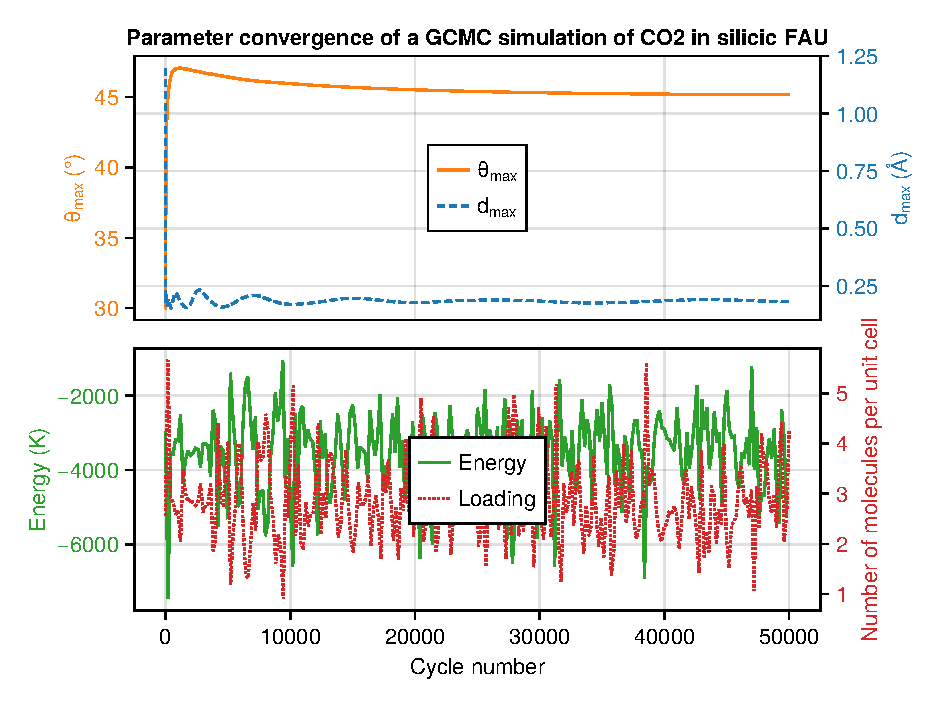
\includegraphics[width=\linewidth]{figures/gcmc/parameterconvergence.pdf}

	\caption{Evolution of $d_{\max}$, $\theta_{\max}$, the energy and the number of molecules during a Grand Canonical Monte Carlo simulation of \ce{CO_2} in silicic FAU at \qty{300}K and \qty{50}{MPa}. The values for the energy and the loading are represented with one point per \num{200} cycles, averaging the corresponding values.}\label{fig:parameterconvergence}
\end{figure}

\Cref{fig:parameterconvergence} illustrates the evolution of $d_{\max}$ and $\theta_{\max}$, as well as the corresponding evolution of the energy and the number of molecules, which indicate the global convergence of the simulation. Both parameters $d_{\max}$ and $\theta_{\max}$ converges smoothly towards their optimum. In this particular simulation, the translation move acceptance rate was \num{24.93}\% and for rotation \num{49.87}\%, very close to the targets of respectively \num{25}\% and \num{50}\%.

At the beginning of each step, an MC move is chosen at random. In our simulations, all three moves (translation, rotation and reinsertion) are chosen equiprobably. For the particular case of the movement of monoatomic species, such as most cations in zeolites, the rotation MC move is useless and thus not used, while the reinsertion move collapses to a simple translation with infinite $d_{\max}$, both moves being chosen equiprobably.

The Metropolis-Hastings algorithm thus provides a way to walk through the configuration space. By privileging moves that decrease energy, the system spends more steps in low energy regions; by yet allowing opposite moves sometimes, the scheme ensures that all the configuration space is eventually visited. Hence, the algorithm guarantees ergodicity: in an infinitely long simulation, the fraction of steps spent in a part of the configuration space is proportional to its volume. %Finding the space with the lowest energy, and thus the largest probability and volume, should then simply be a matter of running the simulation long enough for the state to fall in the deepest energy pit.


\subsubsection{Combined aluminium and cation placement} % method of Marie Jeffroy

Specifically in the case cationic zeolites, Marie Jeffroy \cite{Jeffroy} proposes a simulation method to obtain both the placement of cations in the structure and the location of aluminium atoms across the T-sites. This consists in running an MC simulation where the cations are allowed all previously mentioned MC steps, while the aluminiums are only allowed exchanging positions with silicons, or a restart step that randomly positions aluminiums and silicons, both while obeying L\"owenstein's rule as explained in \cref{mariejeffroy_al}.

The statistical ensemble simulated in this setting includes both aluminium and cations, which means that the distribution sampled through such a simulation method represents the equilibrium for both species. From a chemical point of view, this situation is representative of a framework whose synthesis was done with that very cation, and was thermodynamically-driven. While this does correspond to reality in some cases, there is also evidence that the synthesis is kinetically-driven in many other occurences: for such situation, obtaining the aluminium positions from statistical equilibrium is not representative of the actual framework. And in yet other situations, the cation is exchanged post-synthesis, which decorrelates the aluminium placement in the framework from the cation used for adsorption purposes.

Nonetheless, even in those cases, there is no less value in the aluminium placement obtained from such a hybrid strategy than from random sampling of the T-atoms. In fact, by virtue of the added dimensions of the free energy landscape, a kinetically trapped cation may move more freely following the rearrangement of the aluminiums in the structure, which can make the entire simulation converge more efficiently. If not for the hope of obtaining more relevant aluminium placements, this combined strategy remains valuable for its diminished computationally cost compared to parallel tempering, explained later in \cref{paralleltempering}.

Unfortunately, the fact that the framework is not strictly constant as before prevents the use of precomputed energy grid, later discussed in \cref{energygrid}. This was not a problem in the context of [Marie Jeffroy]'s study because the force field they used was such that a silicon-aluminium swap would not change the van der Waals interactions, but this is not the case of most force fields, including the one we use in our study [BoulfelfelSholl2021]. Being unable to precompute the short-term energy contribution of the framework would thus make the simulations significantly slower, tipping the balance against the use of this method.

\subsubsection{Site hopping}

\label{sitehopping}

Cations are free to move in a canonical MC simulation with translation moves, but some reconfigurations can be problematic. In particular, the cations may not have enough energy to overcome the barriers inherent to the structure of the zeolitic framework in any reasonable simulation time. For example, a cation trapped in the site I of a FAU zeolite will never manage escape into a site III in a room-temperature simulation of reasonable length without a reinsertion move: this simply comes from the high activation barrier it needs to overcome while physically moving out of the sodalite cage. Reinsertion moves are thus useful to allow large configuration movements to occur without having to pass through physical energy barriers.

However, reinsertion consists in attempting to displace a cation to a random position in the framework, which, in the vast majority of cases, ends up rejected because it is too energetically unfavourable. A better move would consist in displacing the cation towards a favourable position, to increase the likelihood of the move being accepted: this is called biasing, which requires unbiasing the acceptation rate to maintain micro-reversibility.

Taking this idea to the extreme, all cations can be forced to sit on one of a fixed set of possible positions, called a site, and to only move by hopping onto another of these positions, irrespective of the distance with the previous position. One hop is then accepted or rejected based on the Metropolis-Hastings criterion, like any other MC simulation. This ``site hopping'' approach entirely bypasses the issue of spatial energy barrier since the cations directly hop onto a site, without having to move through an unfavourable region to access it. Hence, it makes this kind of simulation particularly well adapted to sharp energy landscapes, like that of cations in zeolites.

A major constraint of this simulation method however, is that it requires knowing the cationic sites, which is precisely the purpose of the current development. One could weaken this constraint by allowing many pseudo-sites, for instance taking all the points of a regular grid, but this basically amounts to reverting to reinsertion moves without sites, which defeats the purpose of this protocol. Site hopping is thus useful in the later stages of cation placement, once the positions of the sites have already been identified, in order to evaluate their population.


\subsection{Meta-algorithms}

The previous algorithms allow sampling the configuration space at a fixed temperature. However, even with reinsertion or site hopping, only one particle can move at a time, which is sometimes not enough. For instance, in FAU zeolites, filling both sites I' when starting from an initial configuration where only the central site I is occupied requires that both the central cation move to the edge of the cage and that an external cation be set in the opposite window. Since both movements require passing through an activation barrier, the probability of it happening naturally is low, and thus requires particularly long simulation times to be observed. More generally, collective movements can remain difficult.

To circumvent this issue, the temperature of the simulation can be raised: this mechanically makes all MC steps more likely to be accepted, so higher-energy regions become more reachable. At the same time, a simulation at a hot temperature is much less likely to explore the details of the energy landscape enough to fall into the energy minima of interest, since the accessible configuration space became so much larger. Several meta-algorithms rely on the previously explained algorithms but use different temperatures in different settings, to attempt finding the optimal compromise between wide and detailed explorations.

\subsubsection{Simulated annealing}

The simplest idea consists in running the simulation while smoothly varying the temperature between cold and hot, alternating between increasing and decreasing phases, possibly interspersed with plateaus. This is called simulated annealing, because of the similarity with the recrystallization method used in metallurgy.


% TODO: comment, illustrate.

\subsubsection{Parallel tempering}

\label{paralleltempering}

Simulated annealing explores the configuration space by alternating between cold phases, where the exploration is detailed but localized, and hot phases, where the exploration is fast but superficial. Parallel tempering, also called ``replica exchange'' proposes doing both phases at the same time.

In more detail, a parallel tempering simulation consists in running several MC simulations, the ``replicas'', in parallel, each at a different temperature. The temperatures are taken between room temperature and a hot temperature. An extra MC step is introduced, called the ``exchange'' step, which consists in exchanging the configurations of two replicas with neighbour temperatures. As with any MC step, the Metropolis-Hastings algorithm ensures that the exchange is accepted only if the difference of energy resulting from this exchange is not too high: as a consequence, for the exchange step to be accepted regularly, the temperatures must be taken so that the typical energies of the system between neighbour temperatures overlap, as shown on [FIGURE].

In this strategy, the coldest simulation is constantly exploring a local free energy minimum, while the hottest simulation easily accepts MC moves and thus walks through the entire configuration space. By exchanging configurations, new configurations regularly trickle down from the hot simulations to the colder ones, while the general Metropolis-Hastings strategy ensures convergence towards a global minimum. It is also more efficient than simulated annealing since the exploration of the configuration space is not constrained by the small duration of the hot phase. Parallel tempering is therefore the method of choice used to obtain convergence when facing difficult energy landscapes such as the one encountered for cation placement.

Naturally, its main downside is its computational cost, proportional to the number of simulations and thus effectively related to the difference between the highest and the lowest temperatures. The choice of intermediate temperatures must be guided by an initial discovery of the typical energies encountered by system at each temperature, which requires a few dedicated simulations prior to the parallel tempering. Finding the optimal number of simulations requires striking a balance with the proportion of accepted MC exchange steps, whose impact on the overall simulation convergence can be difficult to measure. Additionally, simulations with neighbour temperatures must regularly synchronize to attempt an exchange, which strongly limits the amount of parallelization usable in the implementation of parallel tempering.

\subsubsection{``Shooting star'' methodology}

Previously exposed methods such as simple canonical MC, simulated annealing or parallel tempering focus on making the system (or at least, one of its replicas) reach equilibrium after a certain number of initial steps, so that the rest of the simulation occurs at equilibrium. This is crucial for the problem of sampling the equilibrium distribution of states in general. For the case of cation placement in zeolites however, the observed crystallographic positioning of the cations indicates that this distribution is sharply peaked: only a discrete number of sites can be occupied, and the question is to find their positions and occupancy. As a consequence, we can use another, simpler, strategy, which is potentially less efficient for the actual sampling of the distribution, but can uncover relevant local minima faster.

This new methodology takes the same simulation elements as the ones previously detailed, but arranges them in a different fashion. We call it ``shooting star'' because it can be decomposed into one hot simulation, like the bright head of the meteor, and a series of cold simulations that stem from it, like the cooling incandescent debris left in its wake.

The first element is the exploration of the phase space. In order to fully explore it, a naive approach consists in doing steps, each of which randomly reinserts a particle in the system. Without the possibility for step rejection, this leads to sampling extremely unlikely states almost all the time however. We propose to perform global exploration by simply running a canonical MC simulation at a very high temperature, for instance \qty{2000}{K}. Such an approach makes most kinetic obstacles irrelevant, but still prevents absurd configurations like when two atoms collide. This MC simulation is simply called the hot simulation.

The second element is the local minima exploration, which is grafted onto the previous one: every $\Delta_{\text{spawn}}$ cycles of the hot simulation, a snapshot of its current configuration is taken and used as the starting point for a cold simulation, \textit{i.e.} another canonical MC simulation that runs at room temperature. $\Delta_{\text{spawn}}$ is chosen so that two consecutive starting points should be uncorrelated. The higher the temperature of the hot simulation, the less correlated its consecutive steps are, so $\Delta_{\text{spawn}}$ can actually be very low. Each cold simulation runs for $M_\text{init}$ initial steps, that allow the system to cool down, and $M_\text{prod}$ production steps at the target room temperature.

Similar to the previous accelerated methodologies, only a fraction of the explored states can actually be used to perform statistics. In the case of simulated annealing, it corresponded to the cold regions of the simulation; for parallel tempering, only the coldest replica is useful to obtain statistics at that temperature; for the current methodology, the relevant steps are the production of the cold simulation. The main advantage of the ``shooting star'' protocol resides in the efficient exploration of the configuration space, rooted in the hot simulation that is independent from the cold ones. Conversely, it lacks the physical meaning of simulated annealing -- which is the numerical counterpart to the annealing process used in metallurgy -- or the time-reversibility of parallel tempering and bare canonical MC.

In terms of parameters, the ``shooting star'' method requires choosing $T_\text{hot}$ the hot temperature, $T_\text{cold}$ the cold one, $N_\text{cold}$ the total number of cold simulations to launch, the previously mentioned $M_\text{init}$, $M_\text{prod}$ and $\Delta_\text{spawn}$, as well as the number $N_\text{init}$ of initial steps of the hot simulation before launching the first cold simulation. Of all these parameters, $T_\text{cold}$, $N_\text{init}$ and $N_\text{prod} = M_\text{prod}\times N_\text{cold}$ must also be chosen for a single canonical MC simulation and $\Delta_\text{spawn}$ can always be taken around 100 (its value has little effect on overall performance and quality as long as it is not too low nor too high). The extra parameters $T_\text{hot}$ is equivalent to the hottest temperature used in simulated annealing and parallel tempering. Finally, $M_\text{init}$ must be evaluated by an initial run, similar to how the intermediate temperatures used in parallel tempering are obtained or the slope and plateau lengths of simulated annealing are usually chosen. The complexity of the overall setup is thus similar to that of simulated annealing.


\subsection{Extraction of sites and population from simulation}

\label{siteextraction}

%To perform gas adsorption prediction, what is needed is a model of the cationic zeolite. With this perspective, the previous simulation strategies can be used to simply provide their cation configurations with the lowest energy, in order to obtain such a model.

%It is interesting however to evaluate the ``shooting star'' methodology as a new general meta-algorithm to simulate systems in sharp energy landscapes. In order to do so, we need a comparison point that can assess the validity of the pseudo-simulation obtained by gluing together all the production steps of the cold simulations. Such a comparison point is the experimental cation localization that can be obtained by X-ray diffraction on zeolite samples with known topology and \SiAl ratio.

Assuming we do not know the position of the cation sites, a canonical MC simulation (possibly with ``shooting star'' or another meta-algorithm) yields a sequence of cation configurations sampled at room temperature. This sequence can be flattened into a map of the zeolite framework, with one additional point at each position occupied by a cation in one of the steps. Looking at this map allows qualitatively identifying the crystallographic sites as the zones where the density of points is the highest. In order to get quantitative information on the site localization and population, we devise a clustering algorithm that extracts the sites from the previous density map.

The first step consists in dividing the space by a regular grid, whose voxels have the same angles as the unit cell but possibly different lengths, taken to be closest to a target value around \qty{0.15}{\angstrom}. To each voxel is then attributed the number of cations encountered within, across the recorded simulation cycles. This first step thus bins the density onto a regular grid.

In the second step, the bins are sorted by decreasing order of their value. Each voxel is then taken in order: if it is closer than a set distance to a previously recorded site, then the location of the site is updated as the average of its current position and that of the voxel, weighted by the respective density of both; the density of the voxel is then added to that of the site. Otherwise, if it is far enough from all existing sites (we use a minimum distance of \qty{1.6}{\angstrom}), it is added to the (initially empty) list of recorded sites, along with its density. This yields a series of sites and their respective occupancy. To be more efficient, the main loop early stops when the density of the inquired voxels go below a threshold value, taken as the maximum density of all bins divided by 100: as a consequence, the occupancies are corrected by a multiplicative factor so that the sum of the occupancies of all sites correspond to the number of cations. We note that this should not be required in theory, but it is the necessary fix to a double discretization artifact, once inherent to the MC scheme, and one due to our binning.

We observe slightly better results by sorting the bins according the decreasing order their smoothed counterparts, where smoothing is done by convolving the density map by a small Gaussian, of standard deviation the size of the diagonal of a voxel. Indeed, this erases some small statistical fluctuations that may change the precise order of the voxels.

This initial list of sites is then symmetrized, to obtain a common list of sites irrespective of the aluminium placements. To do so, a strategy similar to the hashing of aluminium placements (explained in \cref{aluminiumhash}) is used: for each site, its image is computed for each symmetry of the framework. If one of the image is too close (we use a minimum distance of \qty{1}{\angstrom}) to one of the previously recorded sites, they are merged; otherwise, the one closest to a fixed arbitrary reference is recorded. Hence, the initial sites are ``folded'' to yield a list of symmetrically unique sites. Those are then ``unfolded'' again by applying all symmetries to obtain the list of all sites in the framework.

The final list of sites is such that for any site, all its symmetric images are also sites, and two sites cannot be closer than \qty{1}{\angstrom}. Note that the minimum distance of \qty{1.6}{\angstrom} used as a minimum between two starting points of initial sites does not necessarily transfer to the final sites, because of both the growing of the initial sites, and because of the merging operated during the ``folding'' part of resymmetrization.

\section{Results}

\begin{figure}
	{\centering
	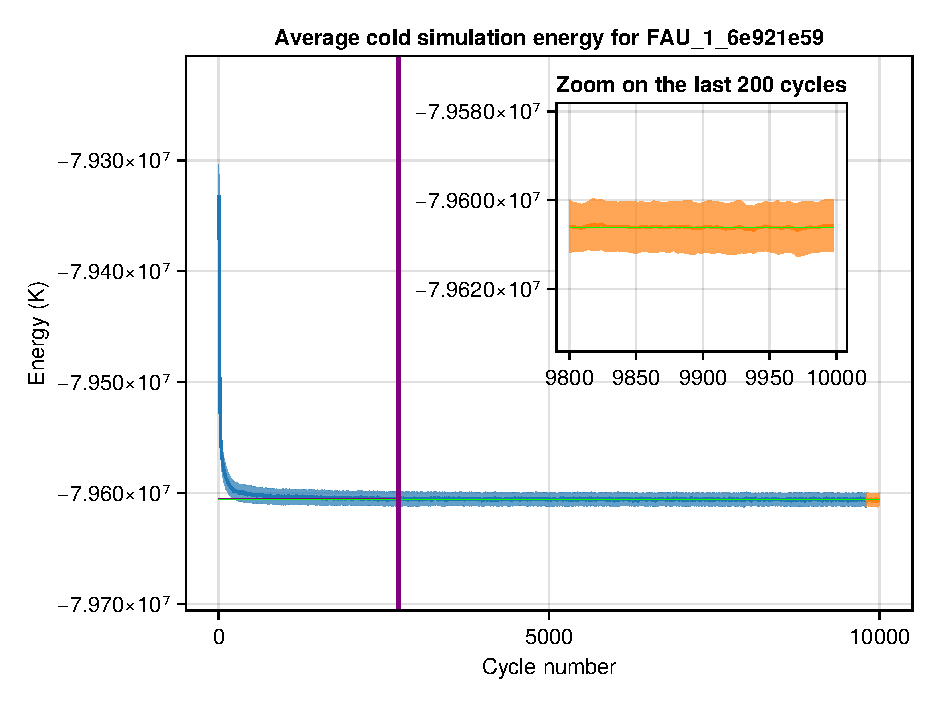
\includegraphics[width=\columnwidth]{figures/cations/convergenceFAUshootingstar.pdf}
	\caption{Convergence of the ``shooting star'' simulation of \ce{Na^+} in FAU with $\SiAl = 1$\\}\label{fig:convergenceFAUshootingstar}

	\sl The dark blue line represents the average energy of the cold simulations for each cycle number. The light blue halo around it represents plus or minus its standard deviation across the cold simulations. The inset focuses on the production cycles using dark and light orange for the same purpose. The vertical purple line identifies the cycle at which the simulation is estimated to have converged. The thin horizontal green line is the average of the energy of the cold simulations during the production cycles. The thin horizontal purple line is the average energy of the cold simulations at the estimated convergence cycle.}
\end{figure}

This section presents the cation location and population results in the studied zeolites. We focus our attention on the FAU (faujasite) zeolite first, because it is an already well-studied case that highlights the main difficulties encountered when attempting to locate cations.

\subsection{Case study: FAU}

\label{casestudyFAU}

The FAU zeolite is one of the most well-known zeolites used in the industry. It is composed of large cages, of \qty{12}{\angstrom} in diameter, separated by 12-membered rings, and small sodalite cages separated by hexagonal prisms. A detail of FAU with $\SiAl = 1$ is illustrated on \cref{fig:FAUdetail}.

\subsubsection{Site localization}

As previously explained, the sites are located by running ``shooting star'' simulations. We use the force field of \textcite{BoulfelfelSholl2021} with the hot simulation running at \qty{2000}K for \num{20000} cycles after \num{2000} initialization cycles, using both translations and reinsertions (without rotation, since the particles are monoatomic) equiprobably. \num{200} cold simulations spawn, once every \num{100} hot cycles, running for \num{200} production cycles after \num{9800} initialization cycles. Only the production cycles are used to record the density map.

The convergence of the ``shooting star'' simulation can be analyzed on \cref{fig:convergenceFAUshootingstar} in the particular case of \texttt{FAU\_1\_6e921e59}, which is simply the faujasite framework with $\SiAl = 1$ (\texttt{6e921e59} is the hash of the only aluminium placement compatible with L\"owenstein's rule, as explained in \cref{aluminiumhash}). This figure mostly focuses on the initialization cycles of the cold simulations, to study the global convergence of the simulation.

Assuming that the different cold simulations are uncorrelated, the standard deviation of their energy at a fixed cycle number gives an information on the statistical noise of the system, which appears to be approximately constant on the figure. Convergence is assessed based on the lack of evolution of the energy averaged across the cold simulations: the vertical purple line marks the first cycle from which the slope of this average energy (smoothed on a few cycles to avoid artifacts) remains below a target bound.

The vertical separation between the green (final energy) and the purple (convergence energy) horizontal lines is another way to quantify the error on the estimation of the convergence of the simulation. In the current case, the difference is well below the statistical noise, which is a further sign of convergence.

\begin{figure}
	\centering
	\hfill\begin{subfigure}{0.45\columnwidth}
		\centering
		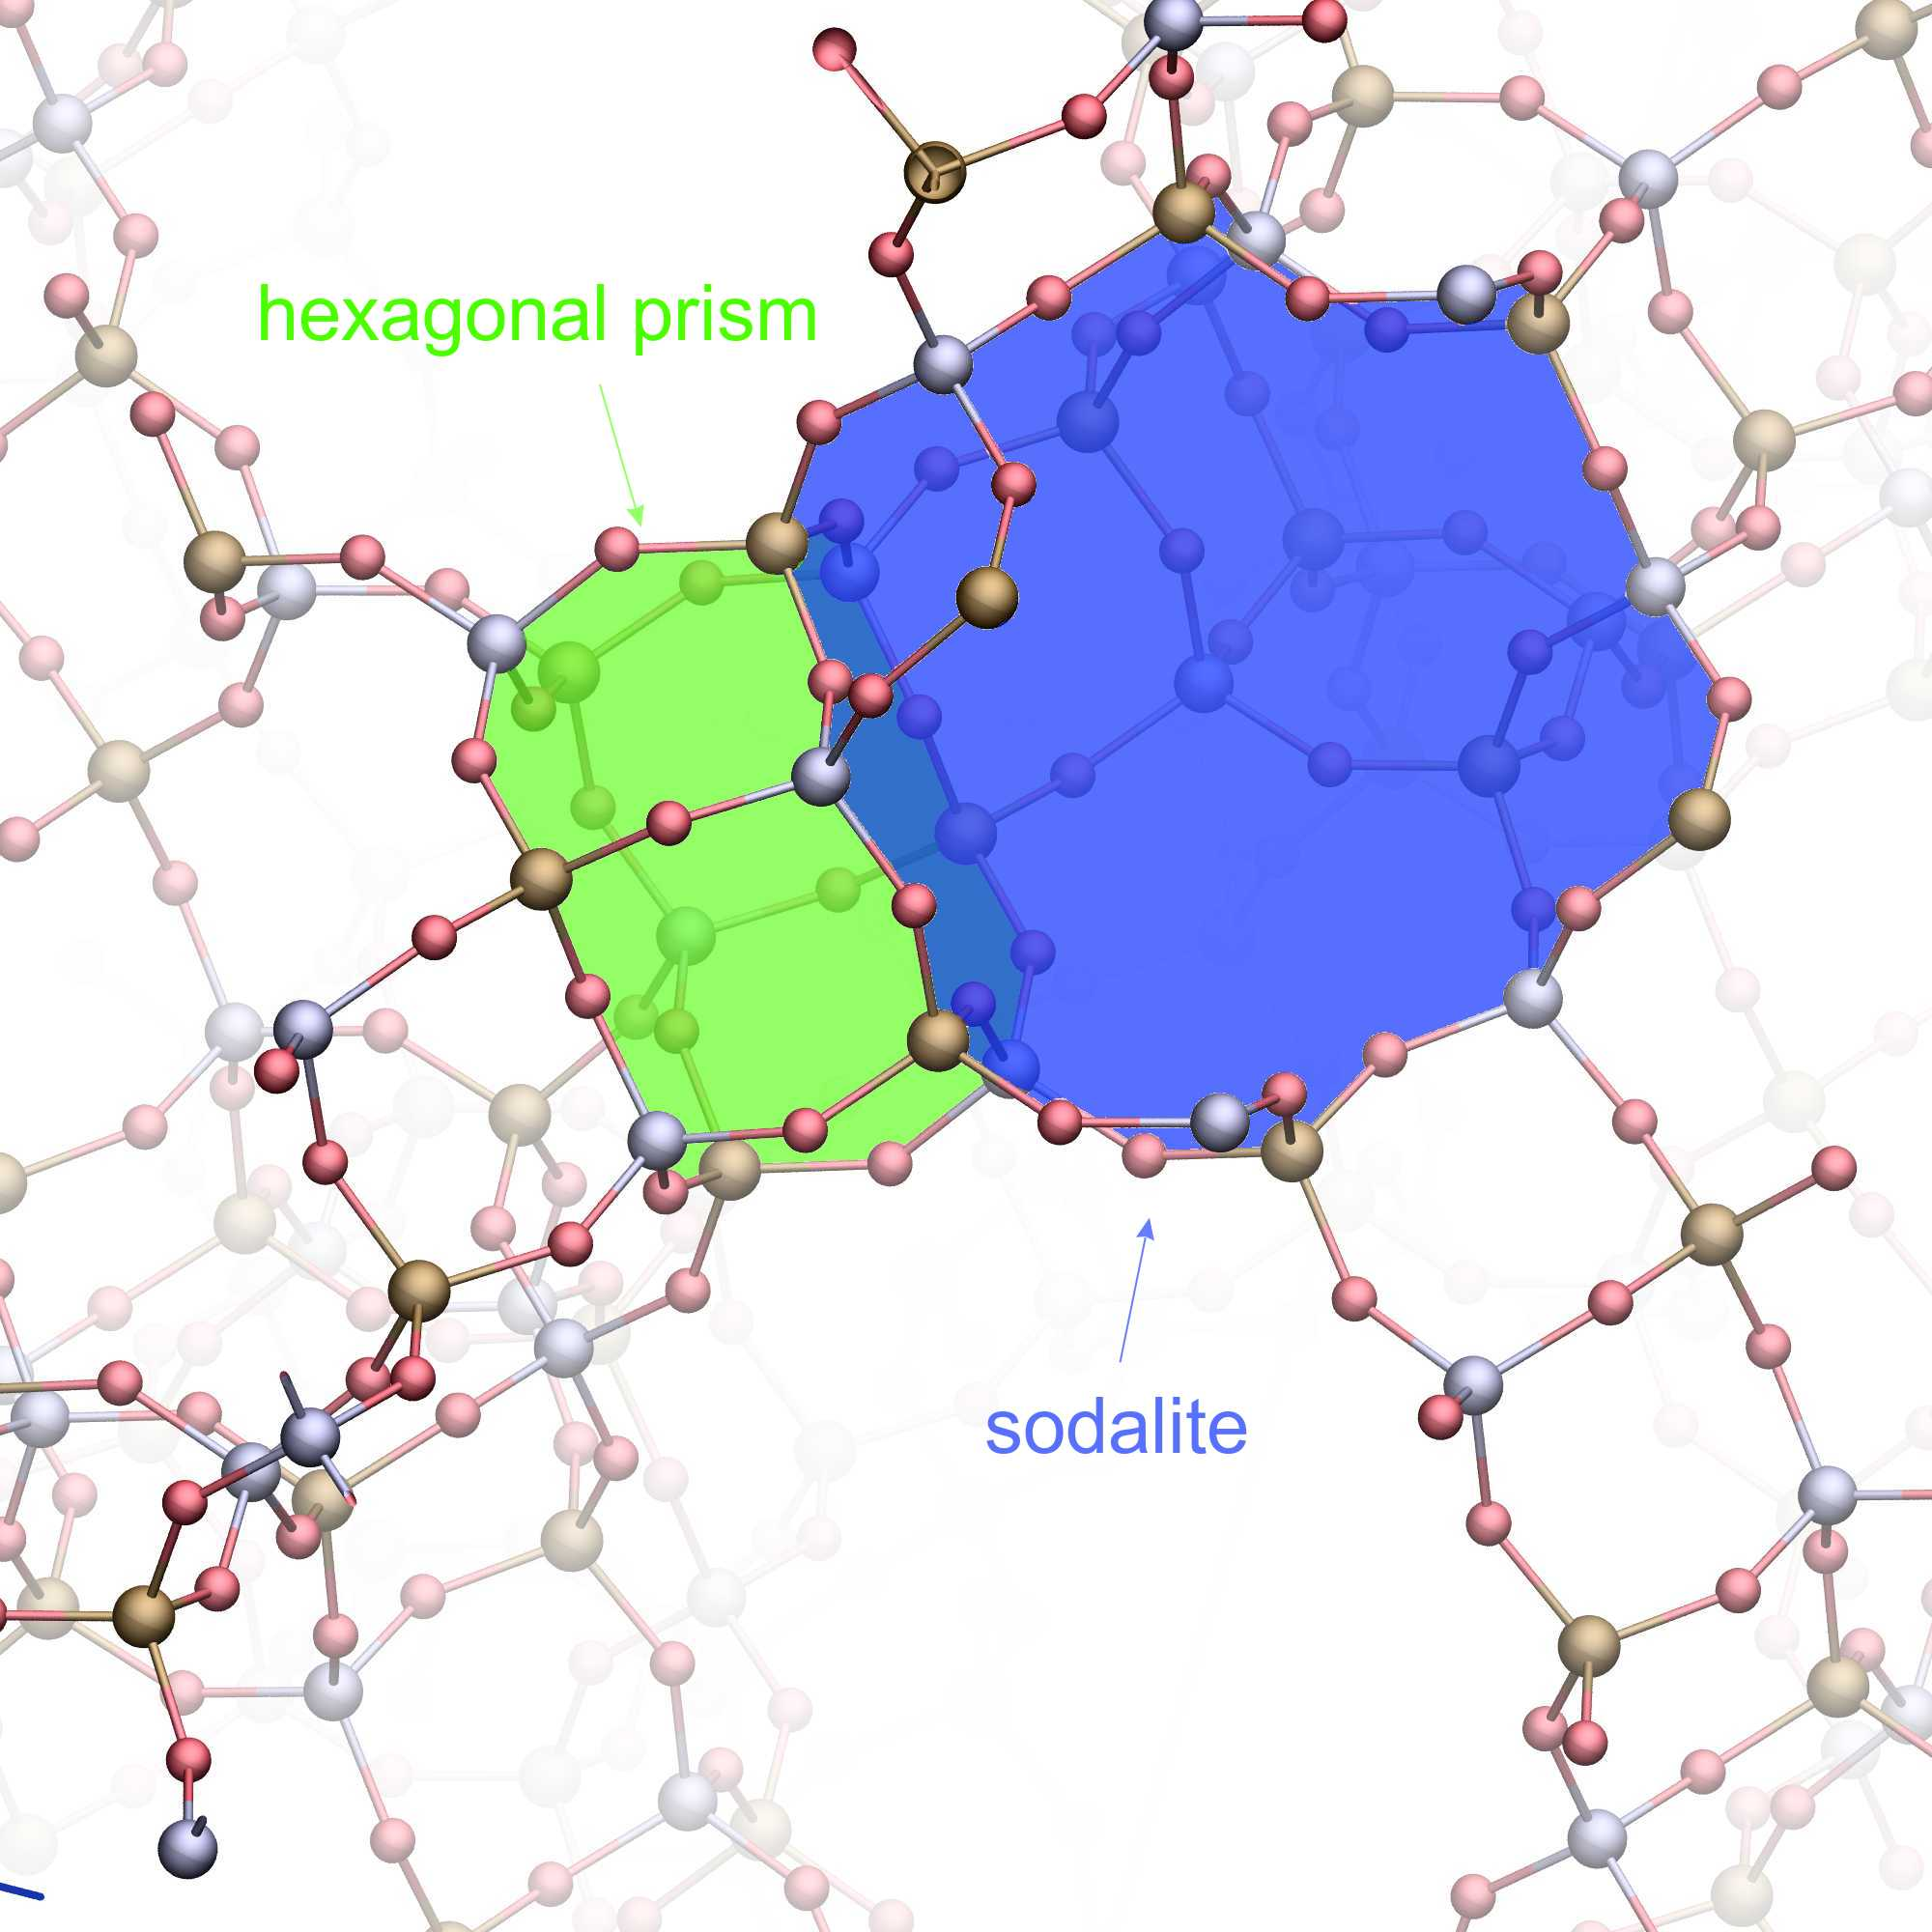
\includegraphics[width=\columnwidth]{figures/cations/FAU1_cages_text.jpg}
		\subcaption{Detail of FAU with annotated cages}\label{fig:FAUdetail}
	\end{subfigure}\hfill%
	\begin{subfigure}{0.45\columnwidth}
		\centering
		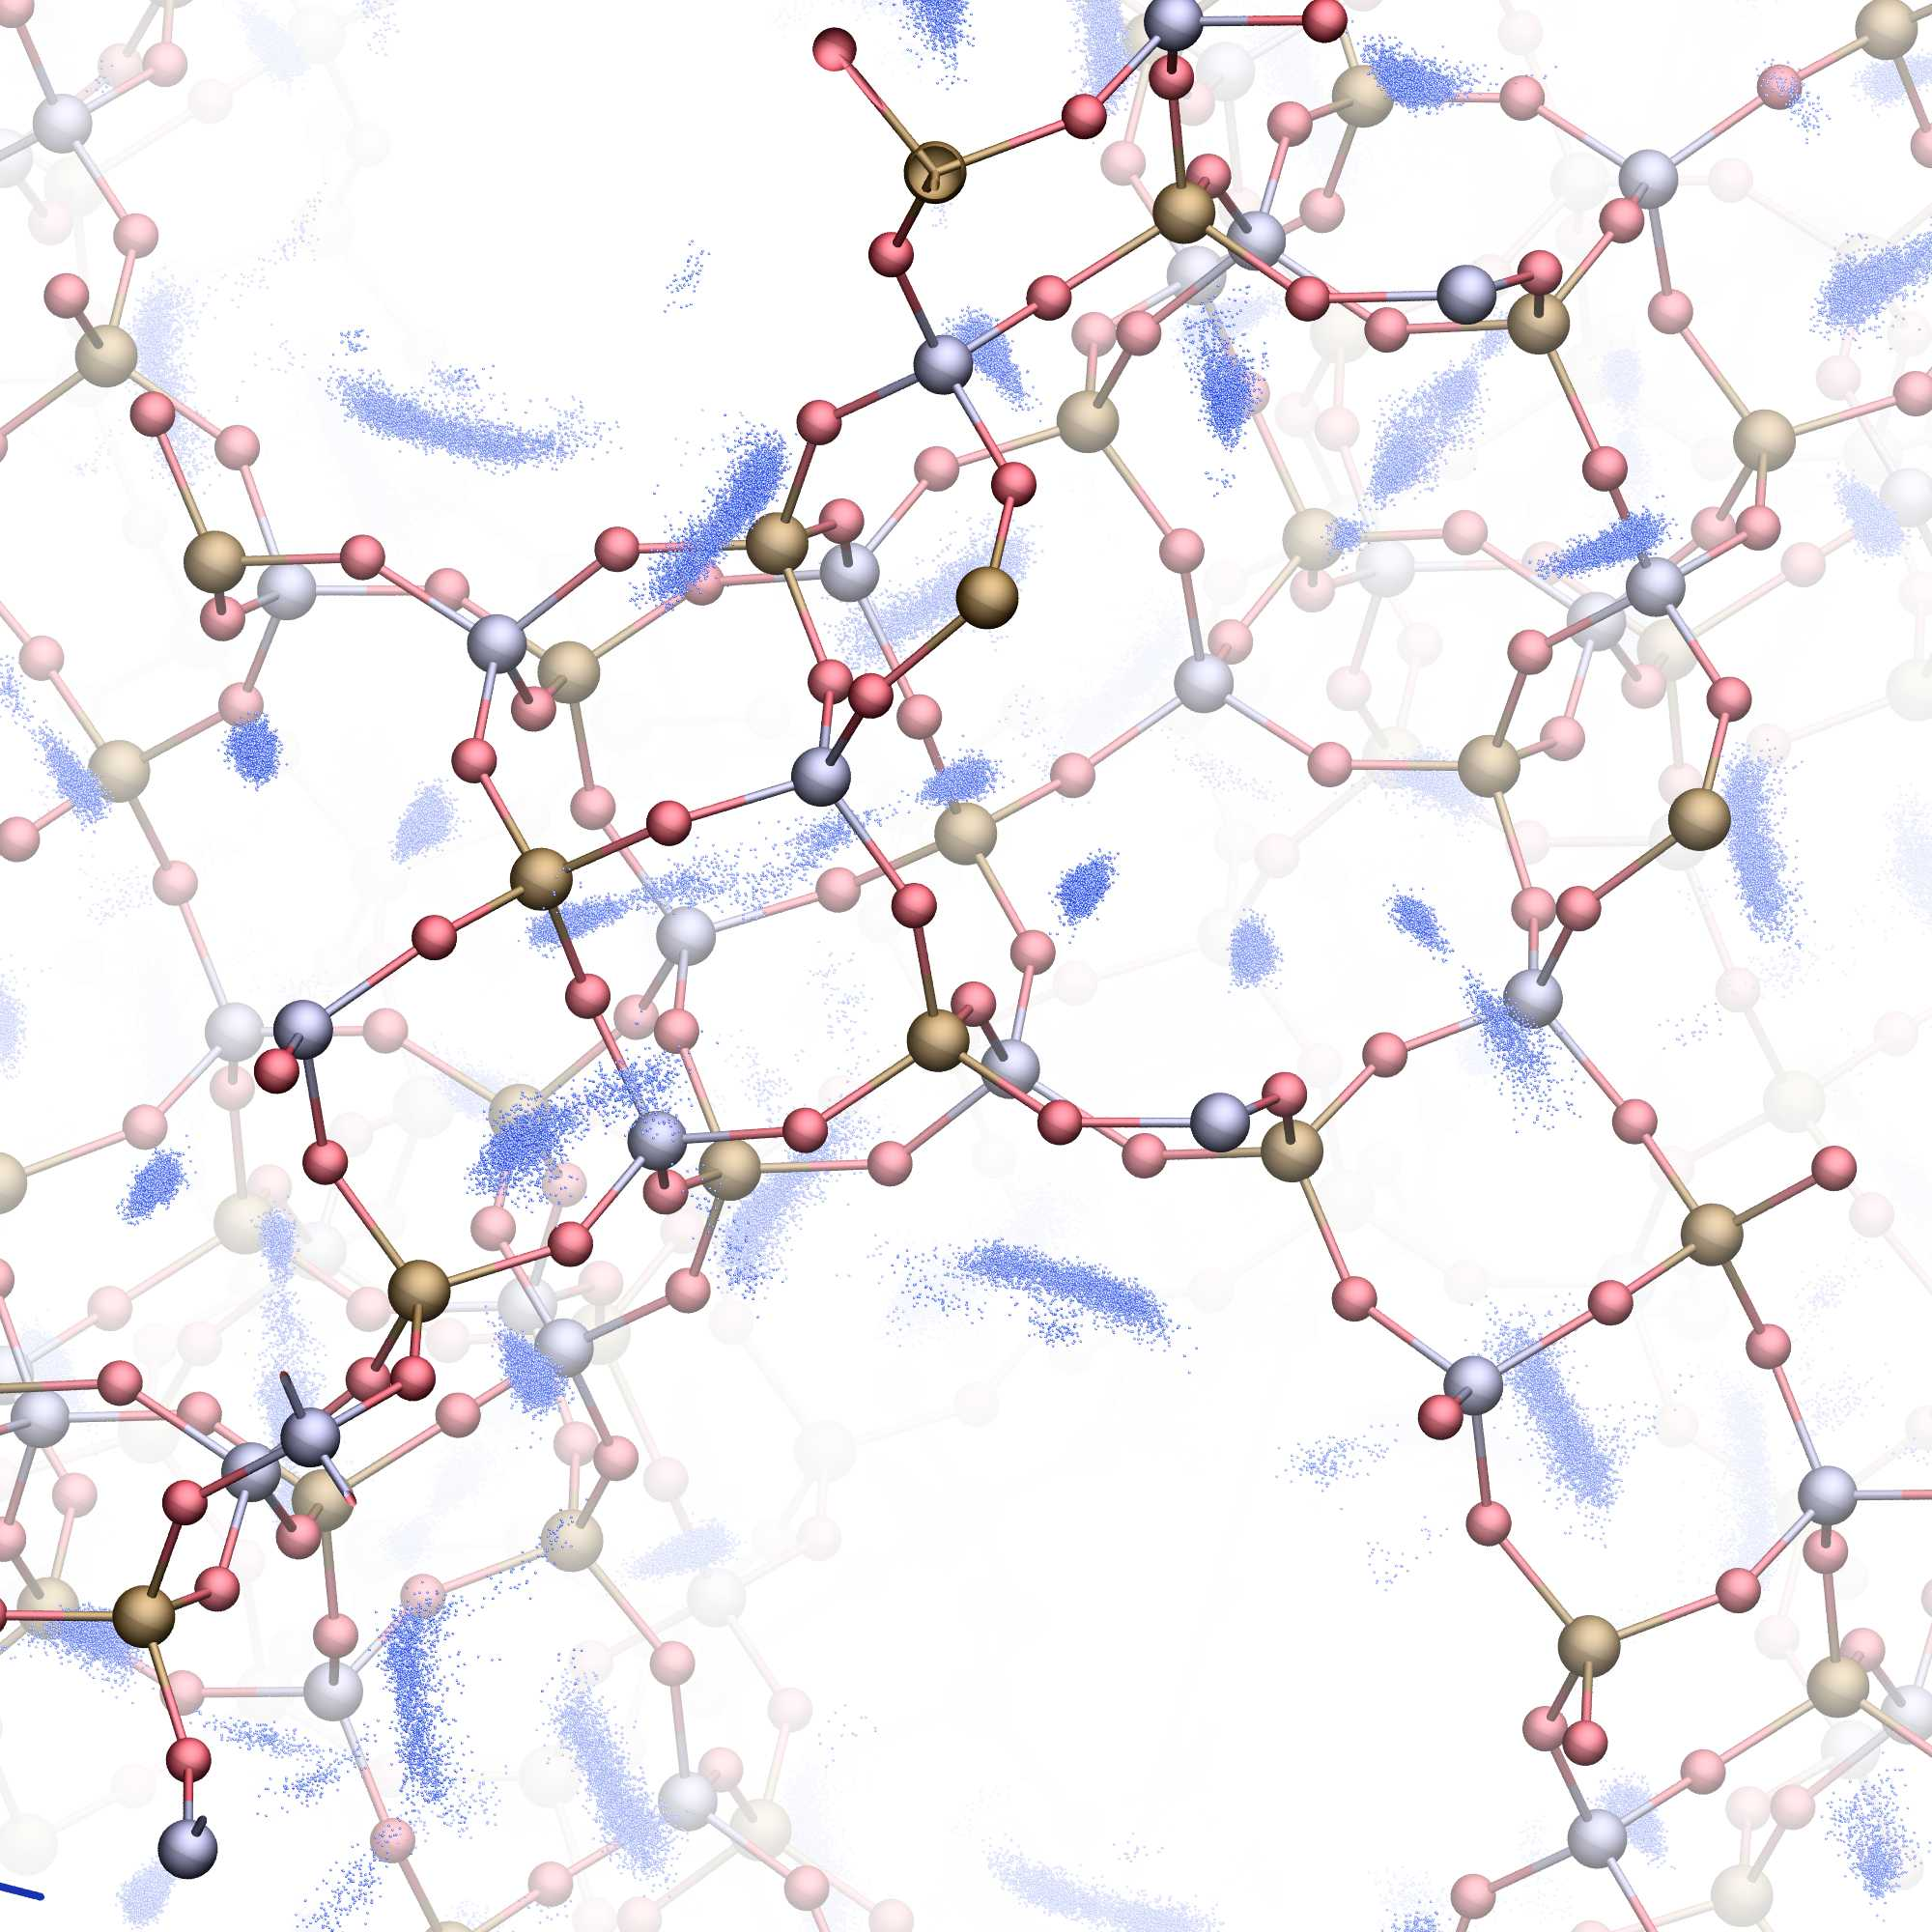
\includegraphics[width=\columnwidth]{figures/cations/FAU1_density.jpg}
		\subcaption{Simulated cation density map}\label{fig:FAUdensity}
	\end{subfigure}\hfill

	\vspace{1em}

	\hfill\begin{subfigure}{0.45\columnwidth}
		\centering
		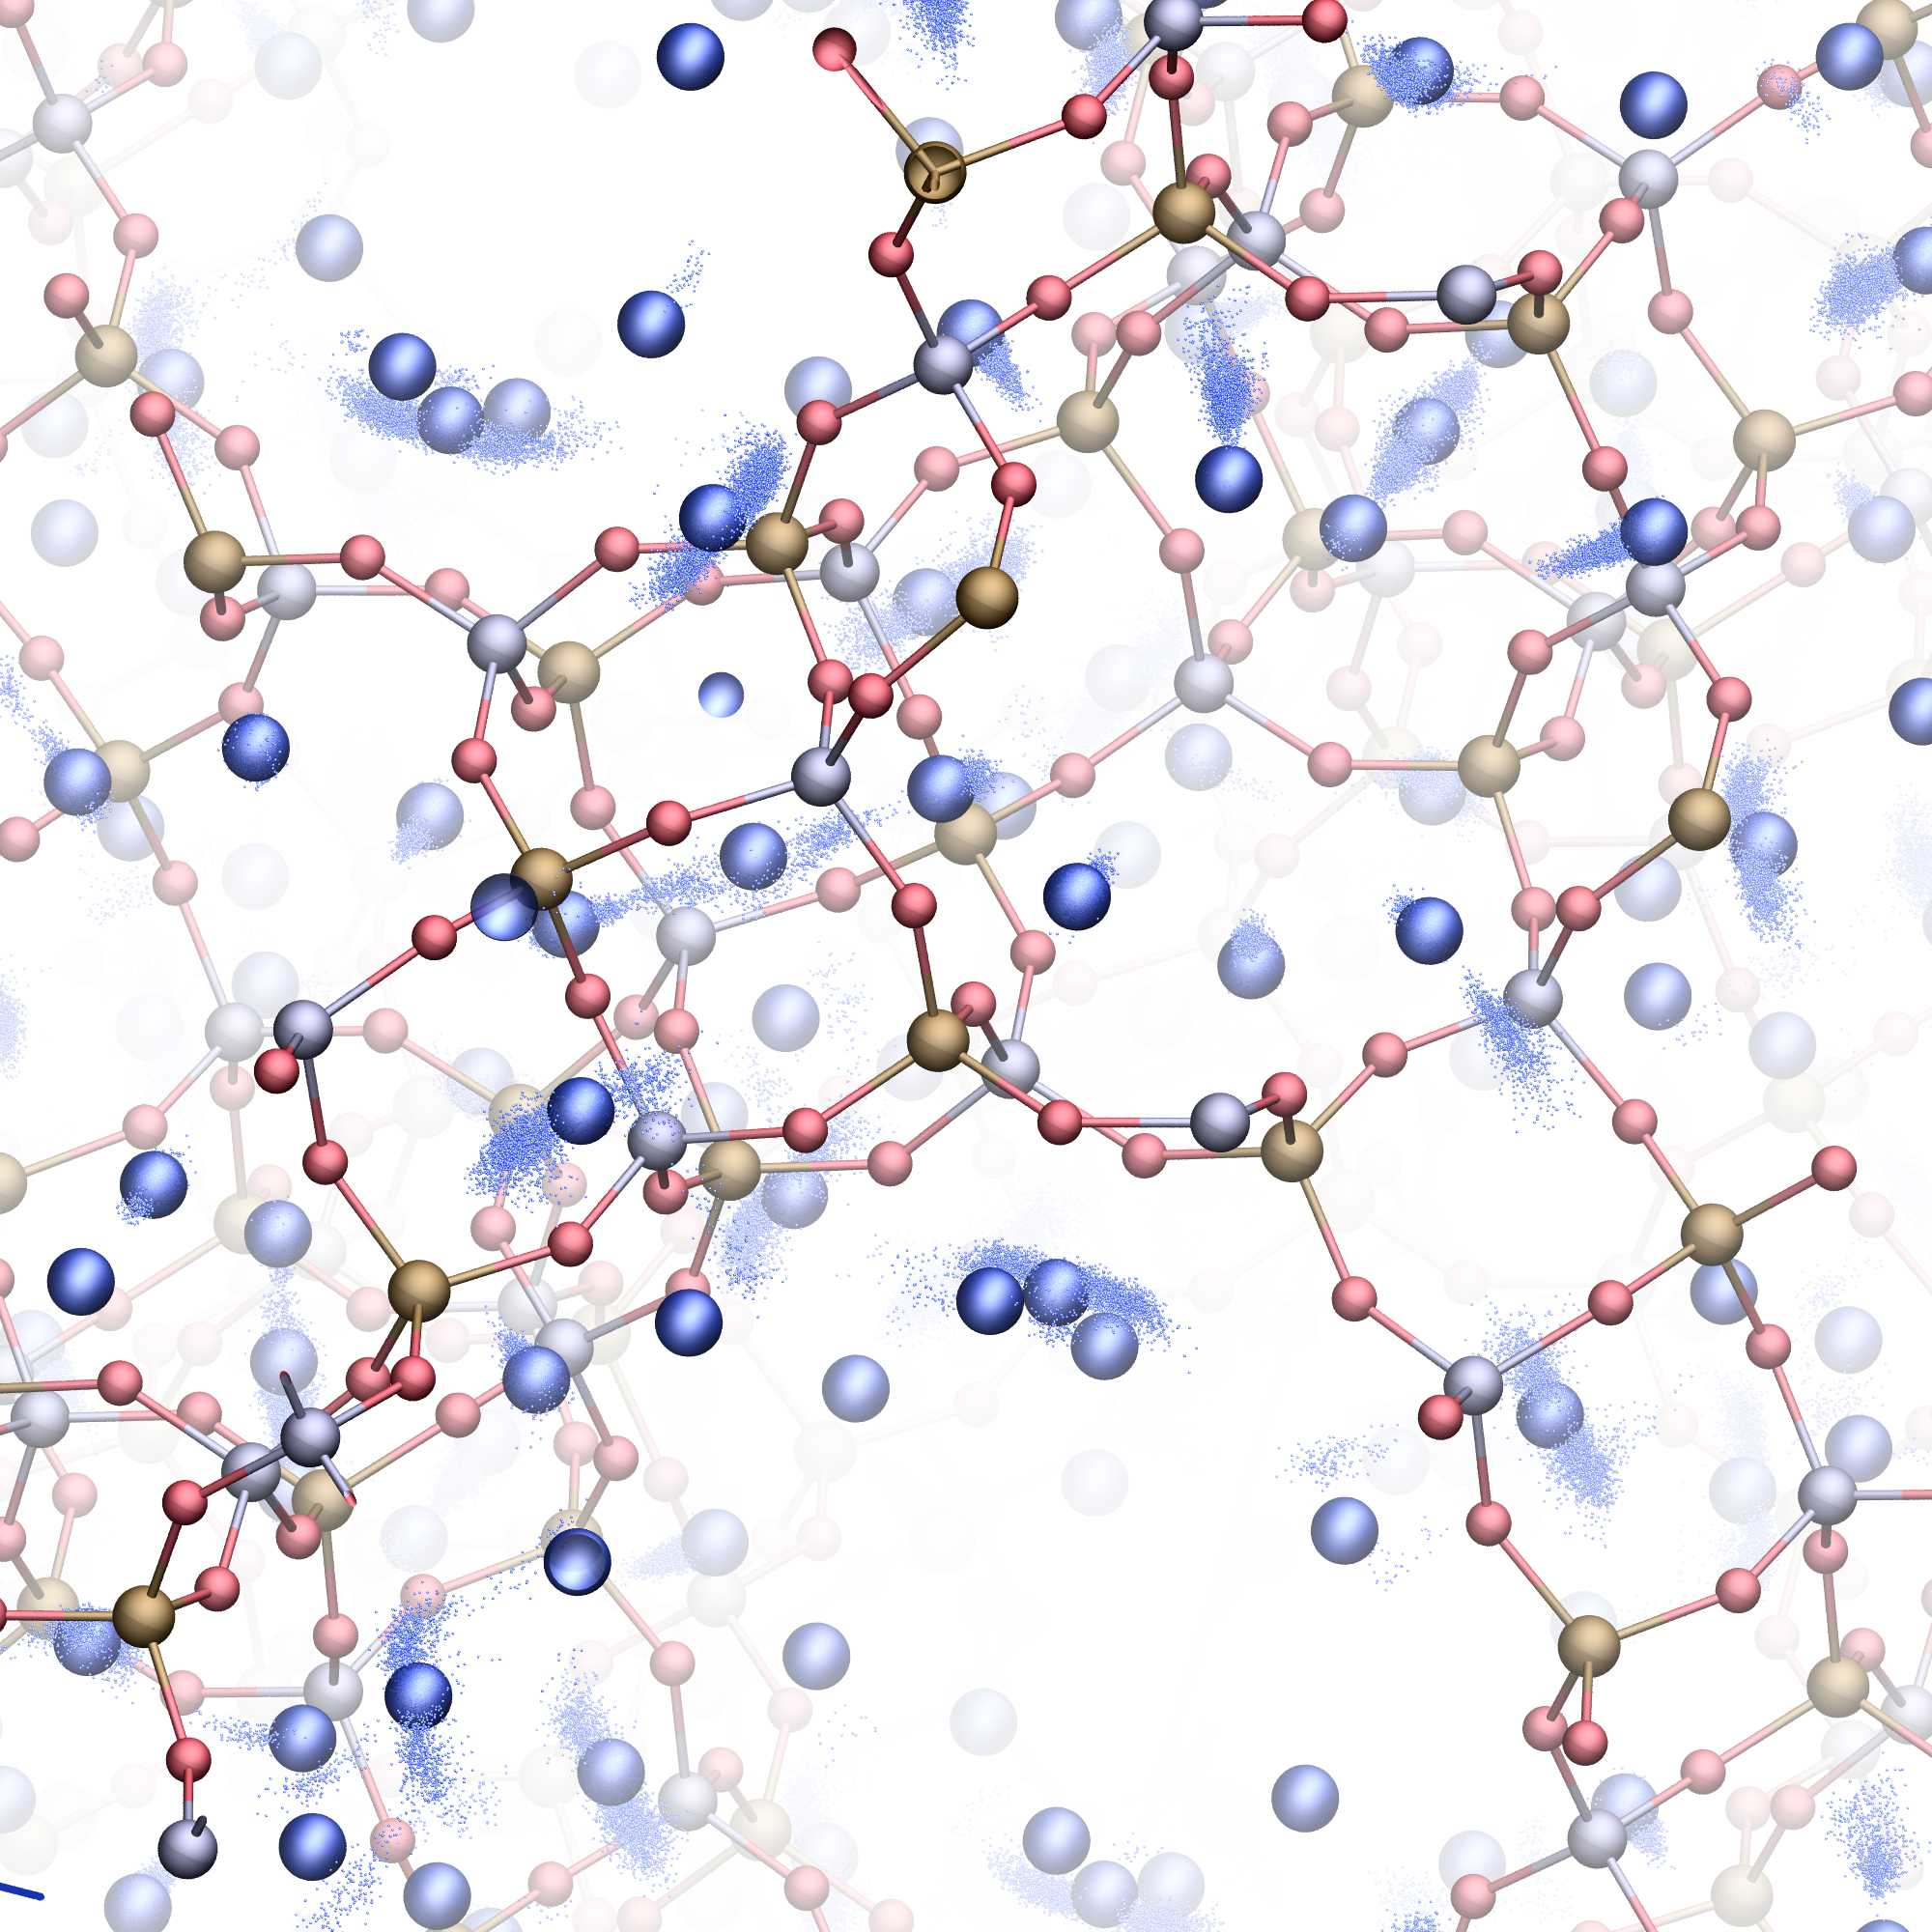
\includegraphics[width=\columnwidth]{figures/cations/FAU1_density_Na.jpg}
		\subcaption{Extraction of sites from the density map}\label{fig:FAUextraction}
	\end{subfigure}\hfill%
	\begin{subfigure}{0.45\columnwidth}
		\centering
		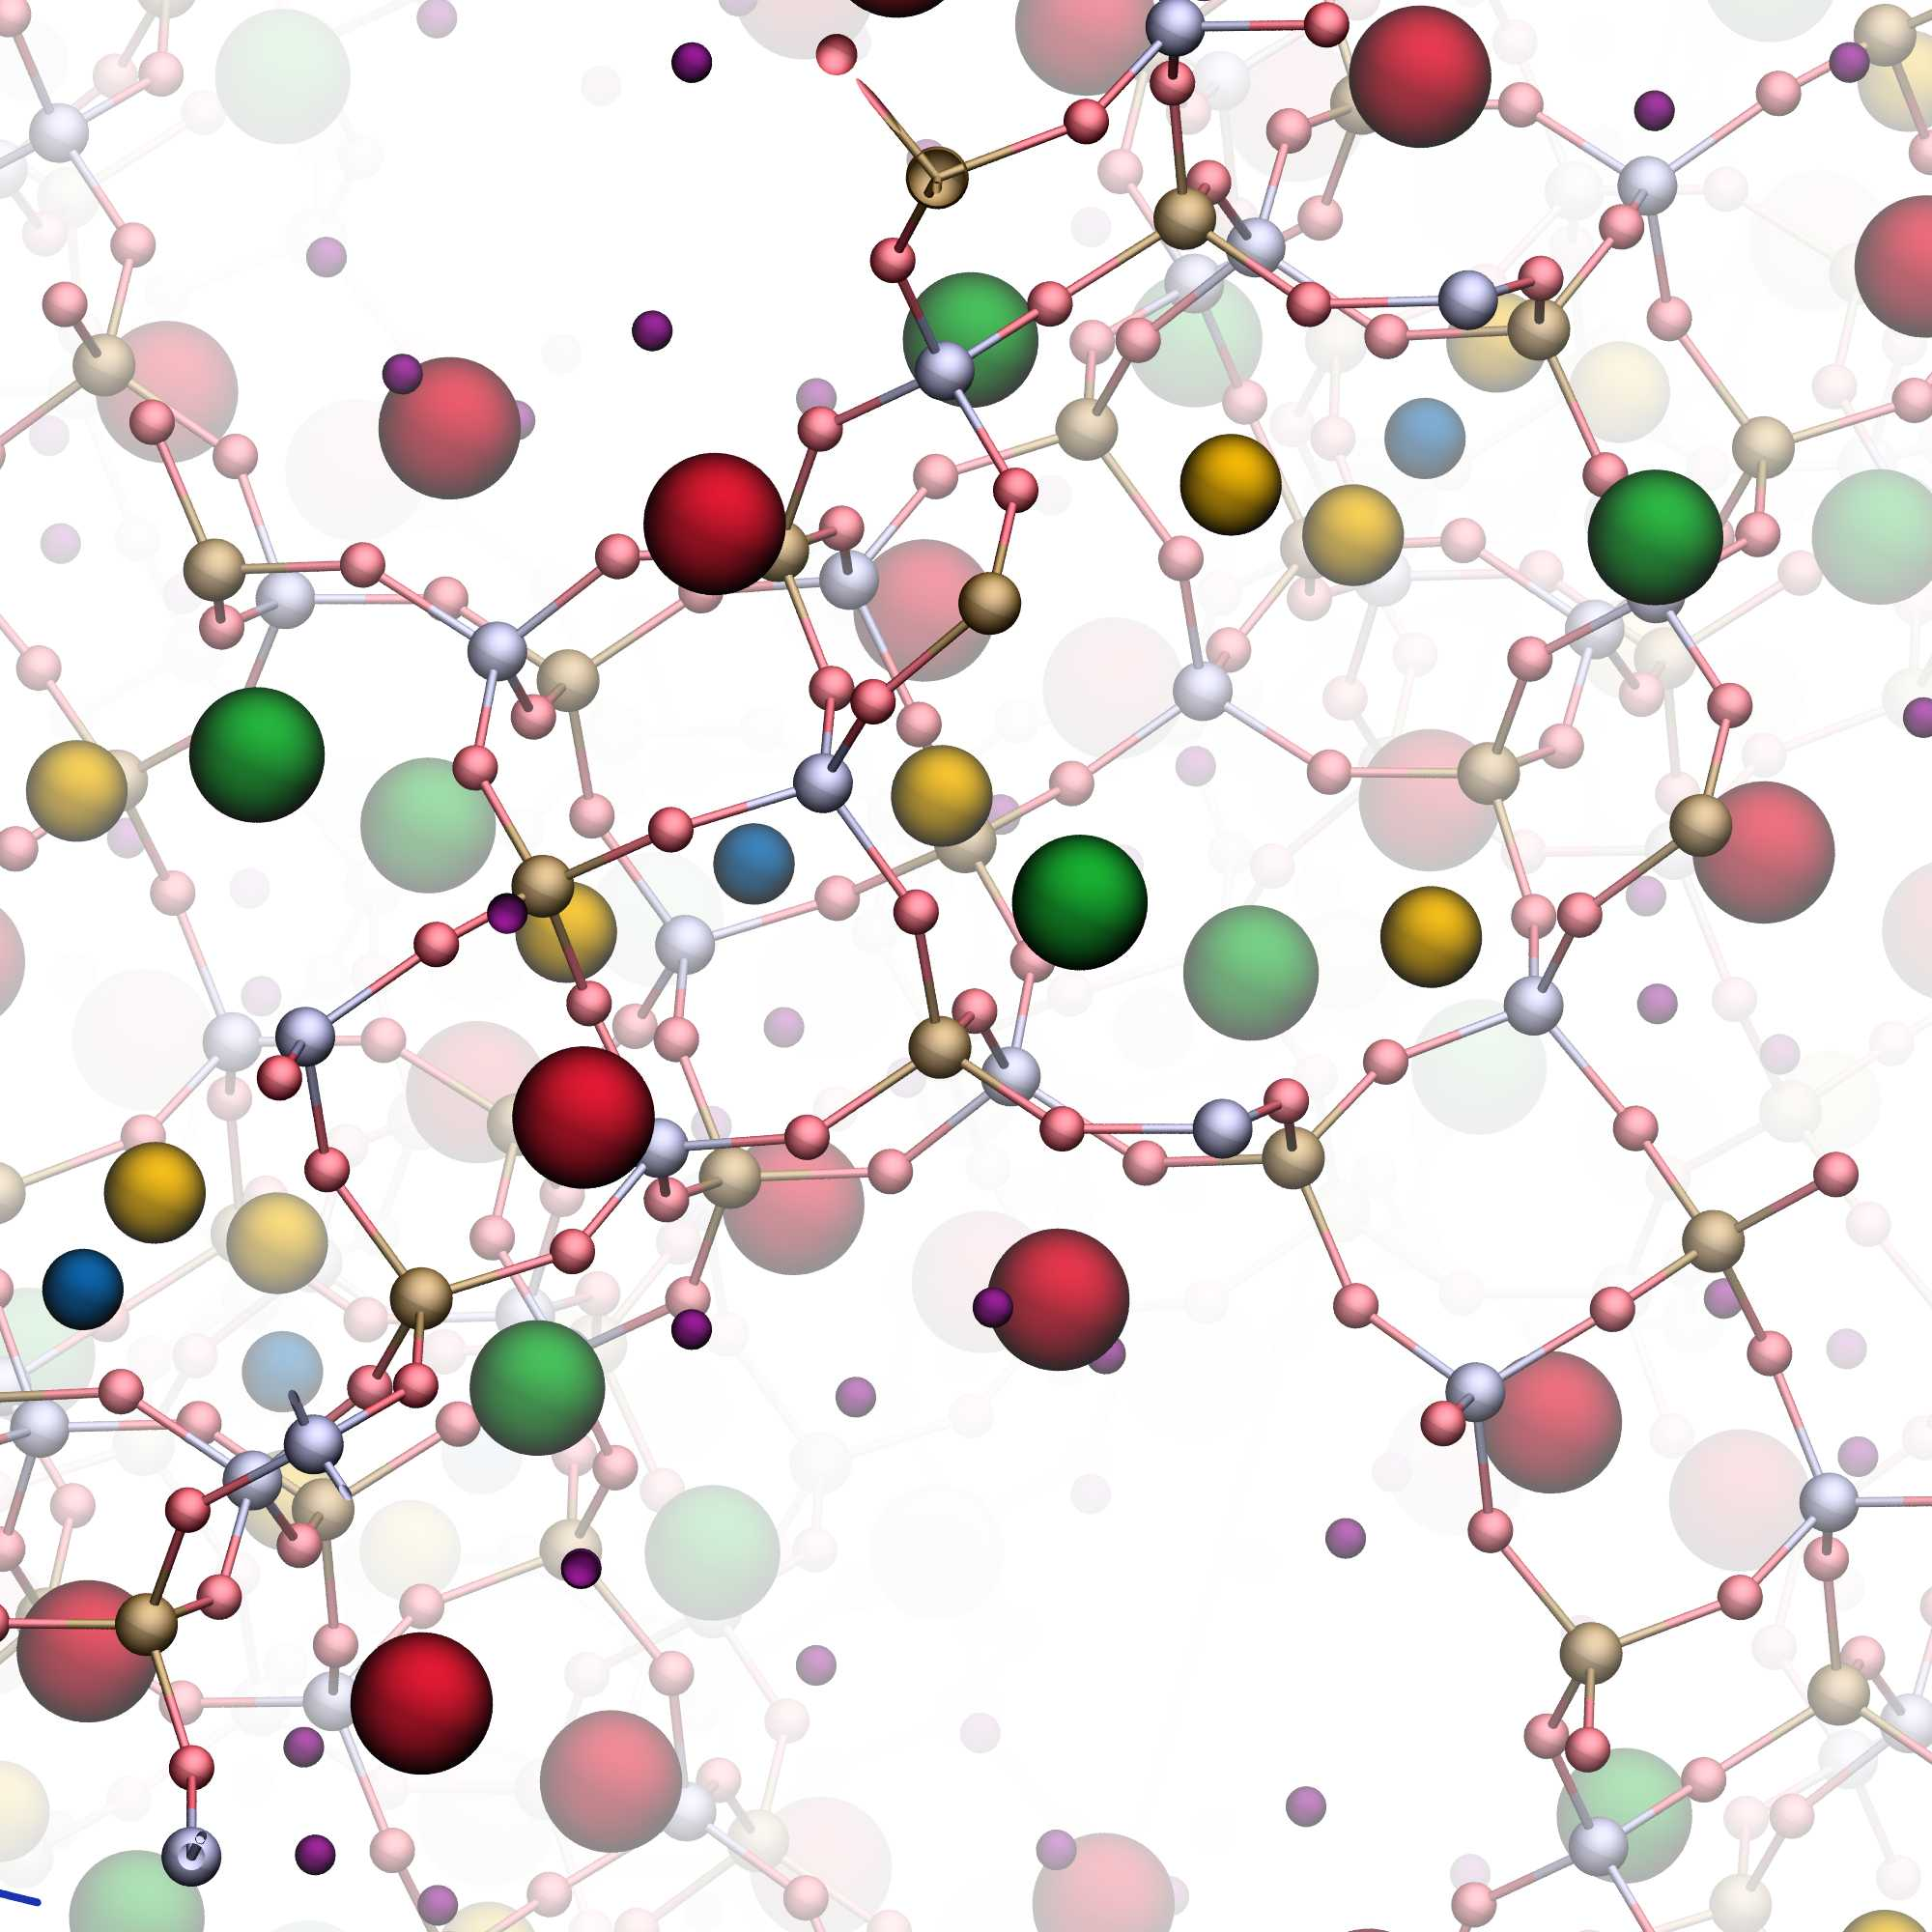
\includegraphics[width=\columnwidth]{figures/cations/FAU1_NaColors.jpg}
		\subcaption{Cationic sites after resymmetrization}\label{fig:FAUsites}
	\end{subfigure}\hfill

	\caption{Cation localization for FAU}\label{fig:FAU}
\end{figure}

Such a simulation runs for all structures corresponding to the reference topology: in the case of FAU, and for all other topologies that can reach $\SiAl = 1$, this means one simulation for $\SiAl = 1$ and six (with six different aluminium placements) for \SiAl equal or approximately equal to \num{1.23}, \num{1.4}, \num{1.7}, \num2, \num3, \num5 and \num{10}, hence \num{43} different ``shooting star'' simulations. The positions of each cation on each recorded cold production cycle across these simulations are flattened into a single density map of the framework, which serves as the basis for the location of cationic sites as explained in \cref{siteextraction}.

\subsubsection{Direct site population}

The site locations are obtained from the flattened density map across different \SiAl ratios, but the resulting occupancies are meaningless. To retrieve site population, the unit cell of the zeolite is divided into volumes centered around each site, such that each point in a volume is closest to the corresponding site than to any other site. This operation is actually the Voronoi decomposition of the crystal space around the sites.

To assert their physical meaning, the Voronoi cells are intersected with solid spheres centered on the corresponding site and of radius \qty{2}{\angstrom}. Hence, any point in space is either in one of the truncated cells, in which case it is associated with a site closer than \qty{2}{\angstrom}, or it is not associated with any site. Once established for a given topology, this map is used for all its corresponding structures (with different \SiAl ratios and aluminium placements). Finding the population of each site from a simulation thus becomes a matter of averaging, across all recorded cycles, the number of cations in the truncated cells associated with each site.

%\renewcommand{\arraystretch}{1.5}

\begin{table}
	\centering
	\begin{tabular}{|c|c|p{9cm}|c|}
		\hline
		\bfseries Cationic & \bfseries Number of & \multicolumn{1}{>{\centering\arraybackslash}m{9cm}|}{\multirow{3}{*}{\bfseries Location}} & \bfseries Color in\\
		\bfseries site & \bfseries sites per && \bfseries figure\\
		\bfseries name & \bfseries unit cell && \bfseries \labelcref{fig:FAUsites}\\\hline
		I & 16 & At the center of the hexagonal prism. & \color{Blue!80!cyan} Blue \\\hline
		&& In the middle of the 6-membered window between &\\
		I'\! & 32 & the hexagonal prism and the sodalite cage, slightly & \color{Dandelion!40!olive} Yellow \\
		&& displaced toward the sodalite cage. &\\\hline
		\multirow{2}{*}{II} & \multirow{2}{*}{32} & In the middle of the 6-membered window between & \multirow{2}{*}{\color{green!50!black} Green}\\
		&& thesodalite cage and the supercage.&\\\hline
		\multirow{2}{*}{III} & \multirow{2}{*}{48} & In the supercage, atop the 4-membered window & \multirow{2}{*}{\color{BrickRed} Red}\\
		&& between the sodalite and the supercage. &\\\hline
		\multirow{2}*{III'\!} & \multirow{2}*{96} & In the supercage, atop the 4-membered window & \multirow{2}*{None}\\
		&& between the hexagonal prism and the supercage. &\\\hline
		&& In the 12-membered window between two supercages, &\\
		J & 96 & atop the oxygen of the 4-membered window between & \color{Plum!60!black} Purple \\
		&& the sodalite and the supercage. & \\\hline
	\end{tabular}
	\caption{Description of cationic sites of FAU}\label{table:FAUsites}
\end{table}

%\begin{table}
%	\centering
%	\begin{tabular}{|c|c|p{9cm}|c|}
%		\hline
%		\bf Cationic & \bf Number of & \multicolumn{1}{>{\centering\arraybackslash}m{9cm}|}{\multirow{3}{*}{\bf Location}} & \bf Color in\\
%		\bf Site & \bf sites per && \bf figure\\
%		\bf name & \bf unit cell && \bf \labelcref{fig:FAUsites}\\\hline
%		I & 16 & At the center of the hexagonal prism. & Blue\\\hline
%		I' & 32 & In the middle of the 6-membered window between the hexagonal prism and the sodalite cage, slightly displaced toward the sodalite cage. & Yellow\\\hline
%		II & 32 & In the middle of the 6-membered window between the sodalite cage and the supercage. & Green\\\hline
%		III & 48 & In the supercage, atop the 4-membered window between the sodalite and the supercage. & Red\\\hline
%		J & 96 & In the 12-membered window between two supercages, atop the oxygen of the 4-membered window between the sodalite and the supercage. & Purple\\\hline
%	\end{tabular}
%	\caption{Description of cationic sites of FAU}\label{table:FAUsites}
%\end{table}

In the literature, the different sites of FAU are well-known and have been given names. Those detected by the previous algorithm are listed in \cref{table:FAUsites} along their usual names and represented in \cref{fig:FAUsites}, using one color per kind of site and with size proportional to their occupancy. Site III' is also mentioned because it is present in other studies, although it was not detected by the algorithm. By contrast, site J is not usually mentioned in studies of faujasite, presumably because it is unoccupied except in the presence of water\autocite{DiLellaFF,WaterFAU}, so its apparition here is possibly an artifact of the force field we use, from \textcite{BoulfelfelSholl2021}.
% The only mention of site J we found was actually in [Marie Jeffroy], who misattributed its nomenclature to [10.1021/ba-1971-0101.ch015], although no mention of site J is present in that reference. There could also possibly be some confusion between the definitions of the two sites, since both correspond to slight displacements of site III, albeit in orthogonal directions.

\begin{figure}
	\centering
	\begin{subfigure}{0.9\linewidth}
		\centering
		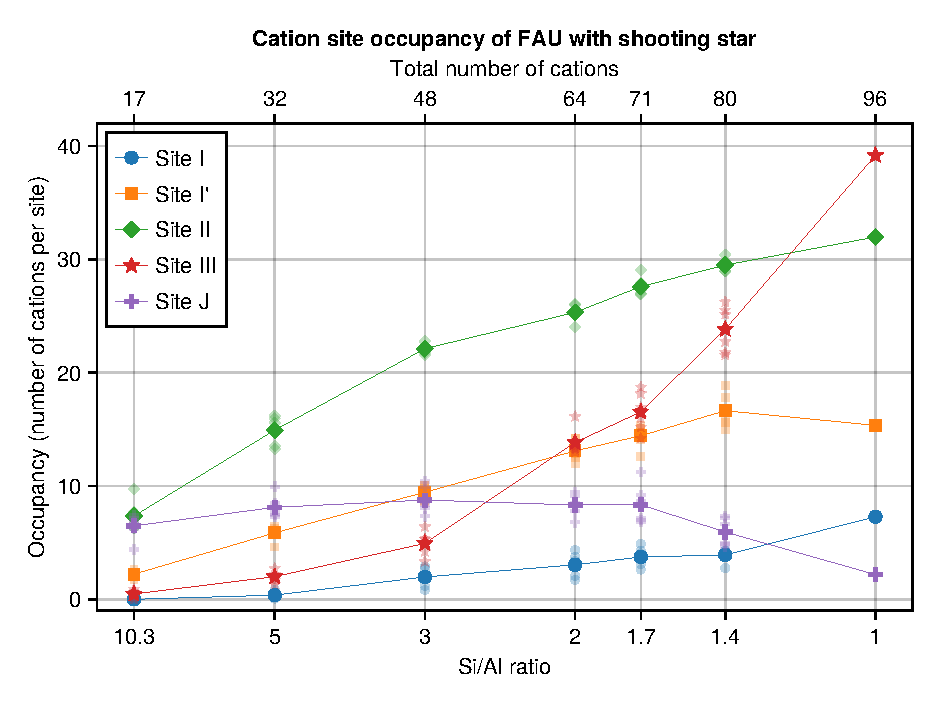
\includegraphics[width=\linewidth]{figures/cations/directsite_FAU.pdf}
		\caption{Data from ``shooting star'' simulation}\label{fig:directsiteFAU}
	\end{subfigure}

	\begin{subfigure}{0.9\linewidth}
		\centering
		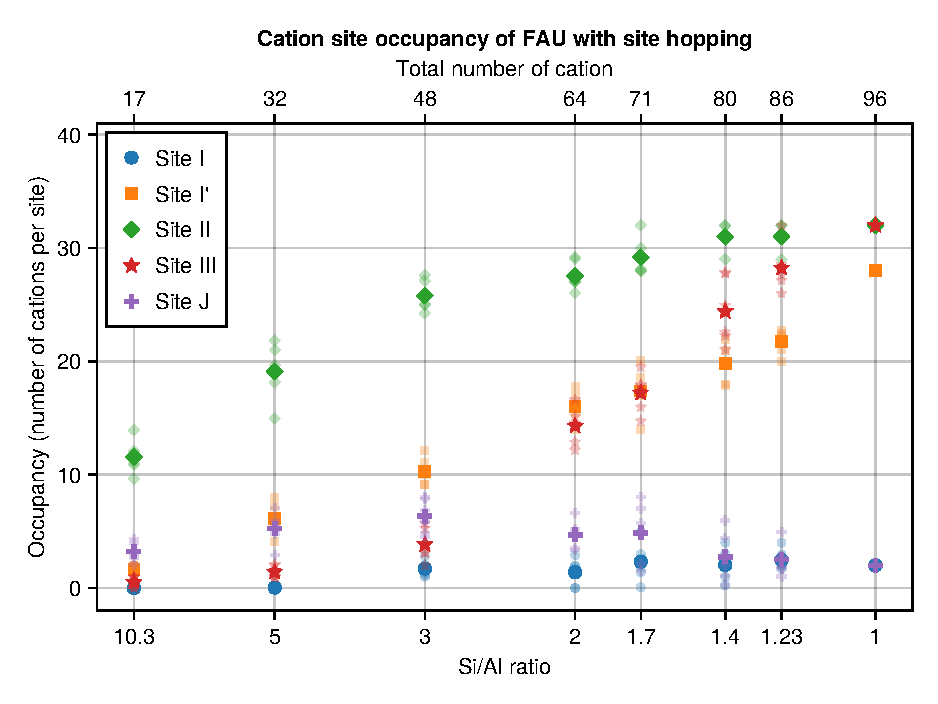
\includegraphics[width=\linewidth]{figures/cations/sitehopping_FAU.pdf}
		\caption{Data from site hopping}\label{fig:sitehoppingFAU}
	\end{subfigure}

	\caption{Population of each site of FAU with force field from \textcite{BoulfelfelSholl2021}}
	
	\sl Transparent symbols indicate the values for each of the 6 explicit aluminium placements.
\end{figure}

With this information, the attribution of the cations to their site can be operated for each cold production cycle of the ``shooting star'' simulation. The average result is presented in \cref{fig:directsiteFAU}.

\subsubsection{Population combined with site hopping}

Alternatively to using the ``shooting star'' simulation results to establish the site population, the resulting site positions can be used to launch a site hopping simulation. Using 1 million production cycles (after 2 million initialization cycles) at \qty{300}K with an output every 1000 production cycles takes up to three minutes per structure and yields a slightly different site population presented in \cref{fig:sitehoppingFAU}.


\begin{figure}
	\centering
	\begin{subfigure}{0.9\linewidth}
		\centering
		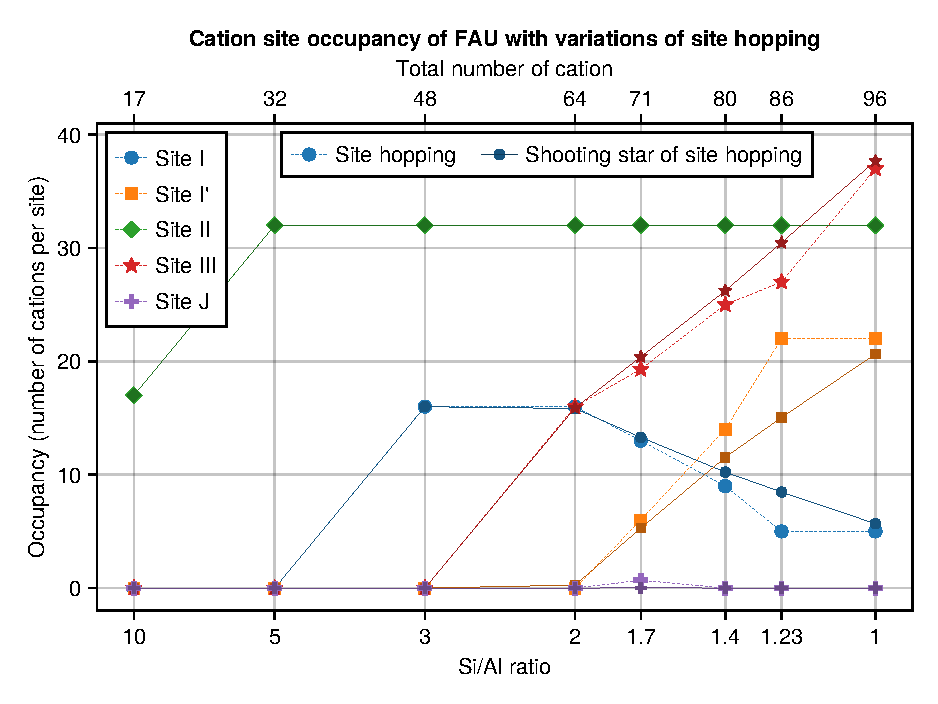
\includegraphics[width=\linewidth]{figures/cations/FAUJeffroyFF_varationssitehopping.pdf}
		\caption{Data from site hopping with and without meta-algorithms}\label{fig:sitehopping_jeffroyFF}
	\end{subfigure}
	
	\begin{subfigure}{0.9\linewidth}
		\centering
		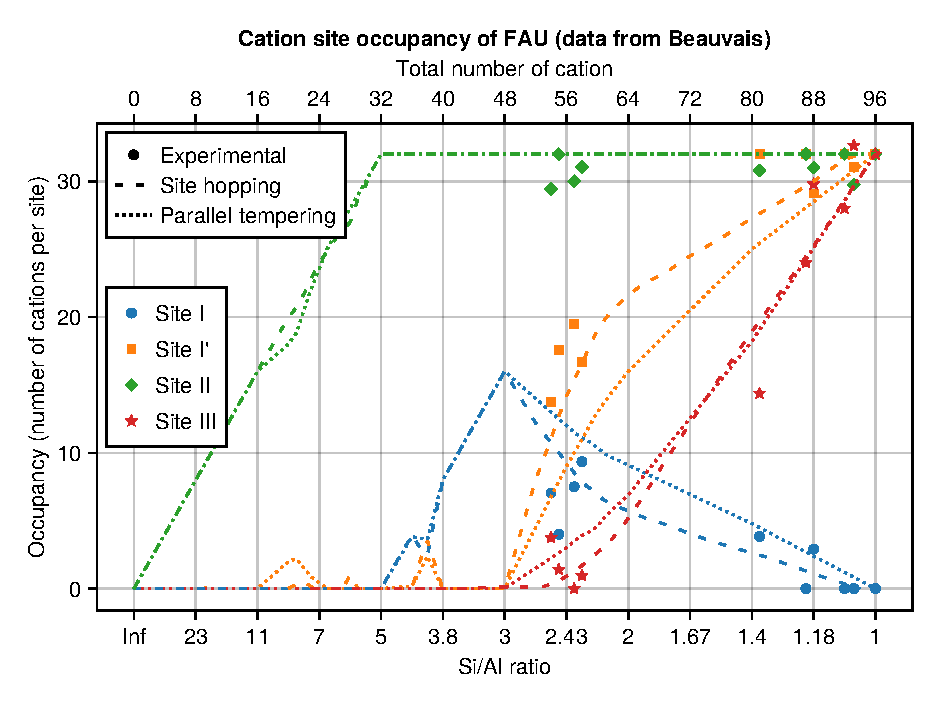
\includegraphics[width=\linewidth]{figures/cations/christele.pdf}
		\caption{Data from Christèle Beauvais's Ph.D. dissertation}\label{fig:christele}
	\end{subfigure}
	
	\caption{Population of each site of FAU with force field from \textcite{DiLellaFF}}
\end{figure}


The main difference comes from the occupation of the sites I' at low \SiAl, which becomes almost maximal for the lowest ratio since since there are 32 sites I'. It appears that the ``shooting star'' simulation alone does not correctly reproduces this trends, while site hopping manages to explore more combinatorial configurations of site occupancy, thus yielding more faithful site populations.

To compare those results with the literature, \cref{fig:christele} reproduces the site population of FAU obtained by Christèle Beauvais in her Ph.D. dissertation, superposing experimental previous works as well as simulation data obtained from both parallel tempering and site hopping, using the force field from \textcite{DiLellaFF}. Site J is not used in that work. Nonetheless, while the general trend of site occupations bears some similarity, the evolution also has some marked differences, notably for site I around $\SiAl = 3$.

I investigated this discrepancy by running a new site hopping simulation, using the same force field by \textcite{DiLellaFF}. The resulting site population, shown in \cref{fig:sitehopping_jeffroyFF} (big light symbols), is indeed more faithful to the original, but still bears a notable population difference for the lowest \SiAl ratios, where site I' fails to reach its expected occupancy of 32. In this force field, the aluminiums and silicons of the framework are represented by an identical T-atom, whose charge depend on the \SiAl ratio, hence there the absence of the transparent symbols indicating the result of each explicit aluminium placement.

Much like any base MC scheme, the site hopping algorithm can be combined with a meta-algorithm to improve its convergence. It is thus possible to run a simulated annealing version, by varying the temperature during the simulation, or even a ``shooting star'' simulation of site hopping. For simulated annealing, the temperatures ramped down \num{400} times, each time starting from \qty{3000}K to \qty{2000}K, then \qty{1000}K, \qty{300}K and finally \qty{300}K again, equally spaced by \num{1000} cycles for each sub-ramp, and recording the site repartition at the end of the last \num{1000} cycles. For the ``shooting star'' variant, this hybrid simulation ran for 2 million hot cycles at \qty{2000}K, spawning a cold simulation every \num{1000} cycles, each running for \num{20000} cycles following \num{1500000} initialization cycles at \qty{300}K.\label{sitehopping_simulatedannealing}

The results are superposed to the simple site hopping computation on \cref{fig:sitehopping_jeffroyFF} (medium symbols for simulated annealing, small dark symbols for ``shooting star''). The two evolutions with meta-algorithm superpose almost exactly, which shows that simulated annealing is complex enough to ensure convergence of site hopping simulations. These evolutions are smoother compared to the bare simulation without meta-algorithm, and show a consistent and marked difference around $\SiAl = 1.23$ in particular: this highlights the interest of using meta-algorithms to ensure proper convergence of even site hopping simulations. It is worth mentioning that the simulated annealing simulation ran to create \cref{fig:sitehopping_jeffroyFF} only takes a few minutes per point, and can be realized in parallel, so the main computational cost of finding the site populations is incurred earlier, when attempting to locate these sites.

These results still differ from those of Christèle Beauvais at low \SiAl, which is unexpected; it might be due to a difference in the exact positions used for the site, or even in the faujasite model used.

\subsubsection{``Shooting star'' simulation calibration}

The temperature of the hot simulation, as well as the inclusion of reinsertion MC moves, was determined by running ``shooting star'' simulations at other temperatures with and without MC moves. Two starting positions of the cations were used, using a single structure with $\SiAl = 2$ hence needing 64 cations: both configurations start by filling the 32 sites II, then the first configuration fills the 32 sites I' (configuration I') while the second fills the 16 sites I and then selects 16 sites III at random (configuration I). As shown on \cref{fig:FAUsites}, every site I is sandwiched between two very close sites I', so a site I' and its neighbor site I cannot be occupied by cations at the same time. These two starting configurations are thus extremes, in the sense that crossing from one to the other requires transitioning through a state where one cation is in a site I' and another in either III or J, which is kinetically costly.

\begin{figure}
	\centering
	\begin{subfigure}{\linewidth}
		\begin{minipage}{0.5\linewidth}
			\centering
			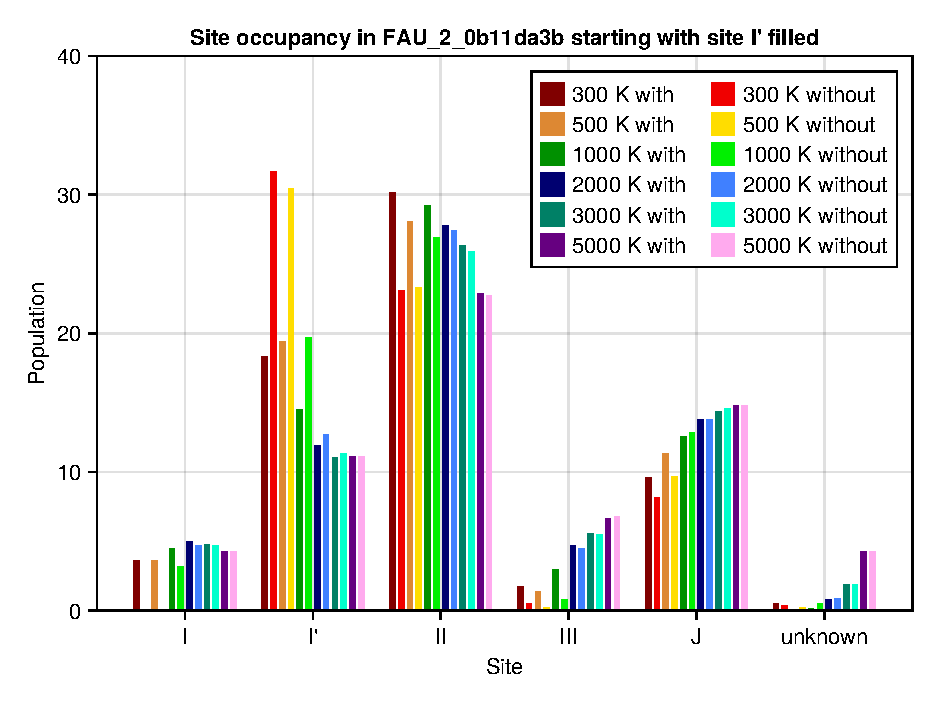
\includegraphics[width=\linewidth]{figures/cations/temperaturecalibration_FAU_2_0b11da3b_logicalstart.pdf}
		\end{minipage}\hfill%
		\begin{minipage}{0.5\linewidth}
			\centering
			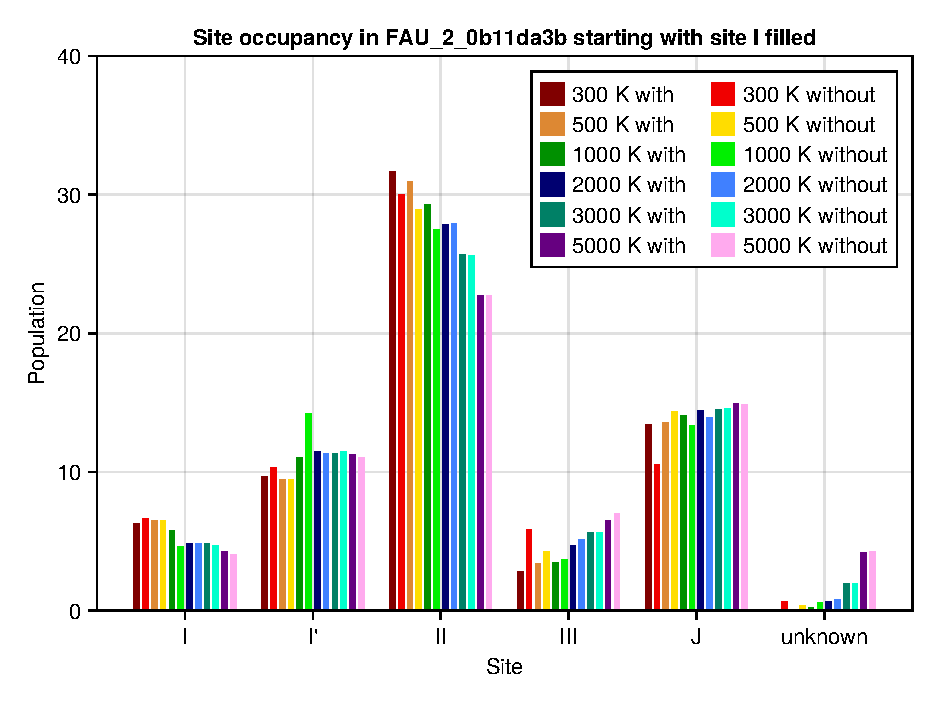
\includegraphics[width=\linewidth]{figures/cations/temperaturecalibration_FAU_2_0b11da3b_absurdstart.pdf}
		\end{minipage}
		\caption{Sites population with force field from \textcite{BoulfelfelSholl2021}}
	\end{subfigure}

	\begin{subfigure}{\linewidth}
		\begin{minipage}{0.5\linewidth}
			\centering
			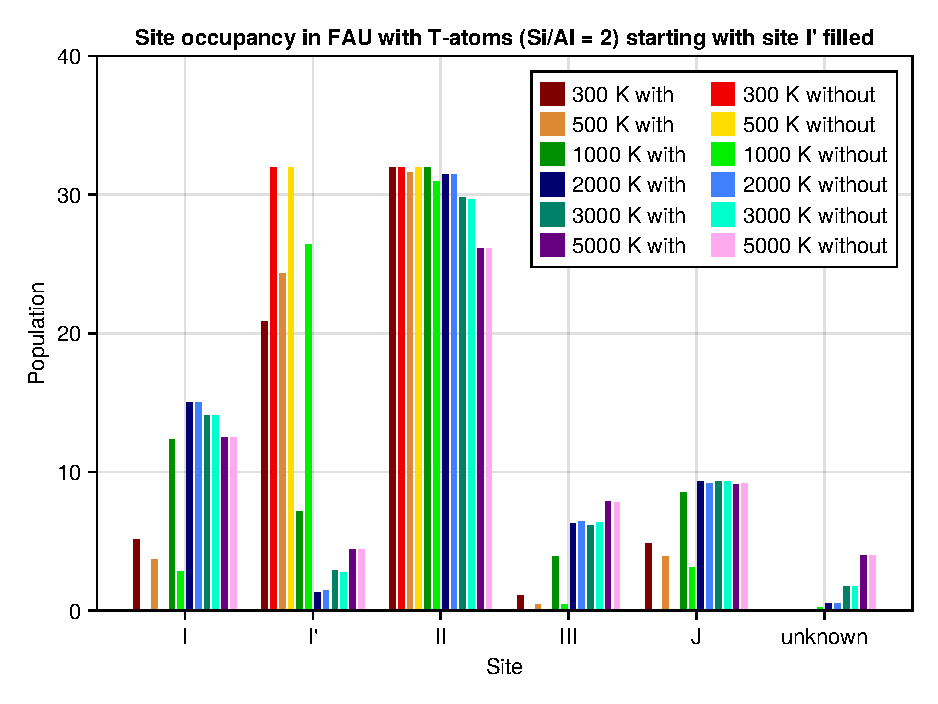
\includegraphics[width=\linewidth]{figures/cations/temperaturecalibration_FAU_T_logicalstart.pdf}
		\end{minipage}\hfill%
		\begin{minipage}{0.5\linewidth}
			\centering
			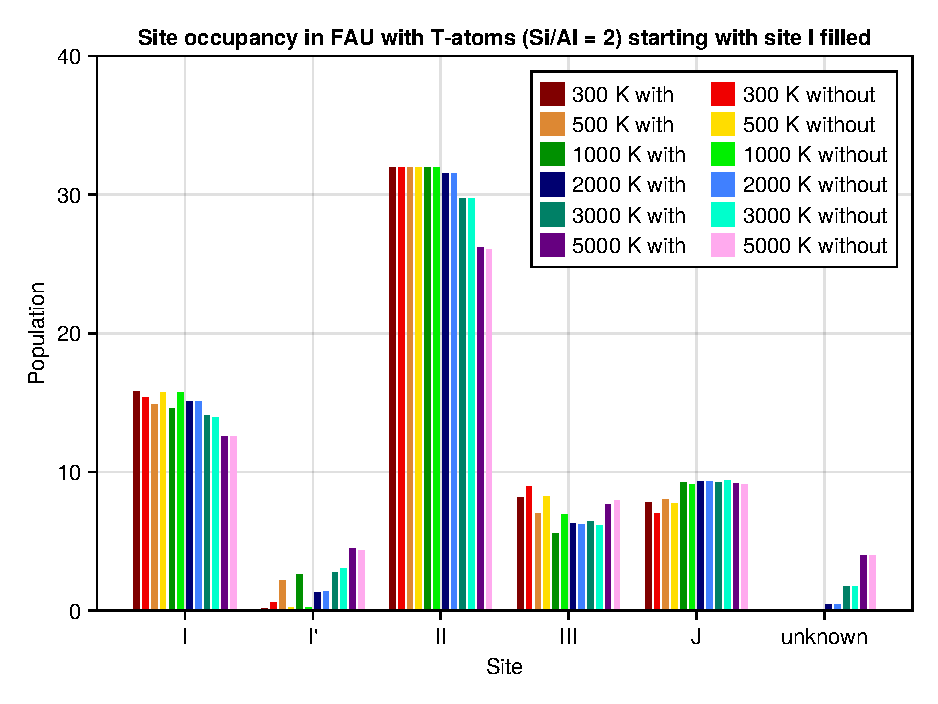
\includegraphics[width=\linewidth]{figures/cations/temperaturecalibration_FAU_T_absurdstart.pdf}
		\end{minipage}
		\caption{Sites population with force field from \textcite{DiLellaFF}}
	\end{subfigure}

	\caption{Hot temperature calibration results for ``shooting star'' simulations.}\label{fig:temperaturecalibration}
	\textsl{``with'' (resp. ``without'') in the legends refers to the presence (resp. absence) of reinsertion moves.}
\end{figure}

The average repartition of cations across the different sites corresponding to these two starting positions are represented on \cref{fig:temperaturecalibration}, using two different force fields. The first one, from \textcite{BoulfelfelSholl2021}, requires having explicit aluminiums so a specific fixed placement was chosen, while the second one, from \textcite{DiLellaFF}, is designed for uniform T-atoms whose properties were set to correspond to the target $\SiAl = 2$.

In both cases, sites I' remain strongly populated for starting configuration I' up to \qty{1000}K without reinsertion moves, much less so with reinsertions, hence the inclusion of these moves appears to significantly increase the convergence of the MC simulations.

The temperature of the hot simulation plays an critical role: at low temperatures, the repartition remains close to the starting position, while at high temperatures the repartition becomes independent of the starting position. This effect is more pronounced on the simulations starting from configuration I', in particular when using the force field by \textcite{DiLellaFF}. The hot temperature of \qty{2000}K was thus chosen because it is the first temperature that shows an identical repartition independent of the starting configuration, while still avoiding having cations out of site (the right-most ``unknown'' bucket in the figure). At that temperature, the influence of the reinsertion moves as negligible, but we kept them for the expected improved convergence overall. The residual cations out of a site have been discarded from the other figures in this section because of their negligible number.


\subsection{Other zeolites}

The methodology developed before is not specific to the FAU zeolite, and can be used on any other structure. At the time of writing, 64 zeolite topologies were automatically investigated by running ``shooting star'' simulations on them at different \SiAl ratios, in order to identify their cationic sites. \Cref{tab:numsites} lists these topologies, along the number of symmetry-wise unique sites identified for each: for example, zeolite FAU has 5 detected unique sites, which are I, I', II, III and J.

\begin{table}
	\centering
\begin{minipage}[t]{0.24\linewidth}
\vspace{0pt}\centering
\begin{tabular}{|c|c|}
\hline
ABW&3\\\hline
AEL&7\\\hline
AFG&6\\\hline
AFO&6\\\hline
AHT&4\\\hline
ANA&2\\\hline
ANO&12\\\hline
AST&1\\\hline
ASV&3\\\hline
ATN&3\\\hline
ATS&7\\\hline
ATV&5\\\hline
AWW&5\\\hline
BOZ&15\\\hline
CAN&2\\\hline
CAS&5
\end{tabular}
\end{minipage}%
\begin{minipage}[t]{0.24\linewidth}
\vspace{0pt}\centering
\begin{tabular}{|c|c|}
CFI&8\\\hline
CHA&4\\\hline
DOH&6\\\hline
DON&12\\\hline
EMT&14\\\hline
EWO&7\\\hline
FAR&8\\\hline
FAU&5\\\hline
FER&8\\\hline
FRA&13\\\hline
GIU&10\\\hline
IFO&8\\\hline
IHW&11\\\hline
IRN&14\\\hline
JRY&6\\\hline
LIO&11
\end{tabular}
\end{minipage}%
\begin{minipage}[t]{0.24\linewidth}
\vspace{0pt}\centering
\begin{tabular}{|c|c|}
LOS&4\\\hline
LTA&2\\\hline
LTJ&2\\\hline
LTL&6\\\hline
MAR&11\\\hline
MEL&19\\\hline
MFI&32\\\hline
MSO&5\\\hline
MTW&8\\\hline
NPT&2\\\hline
NSI&7\\\hline
OBW&6\\\hline
PTT&5\\\hline
RFE&10\\\hline
RTE&5\\\hline
RWY&3
\end{tabular}
\end{minipage}%
\begin{minipage}[t]{0.24\linewidth}
\vspace{0pt}\centering
\begin{tabular}{|c|c|}
SAF&7\\\hline
SAS&3\\\hline
SAT&6\\\hline
SFE&12\\\hline
SFG&22\\\hline
SFN&11\\\hline
SGT&5\\\hline
SOD&1\\\hline
SSF&11\\\hline
TOL&17\\\hline
TON&6\\\hline
TSC&8\\\hline
UFI&8\\\hline
UOZ&4\\\hline
VET&6\\\hline
VFI&4\\\hline
\end{tabular}
\end{minipage}

	\caption{Number of cationic sites identified per investigated zeolite topology}\label{tab:numsites}
\end{table}

These numbers exhibit quite large disparities, between only 1 for AST and SOD to 32 different unique sites for MFI. This can be explained by correlating them with the volume of the asymmetric unit of the framework, that is the volume of its unit cell divided by the number of symmetries of the topology, as illustrated on \cref{fig:sitesvolumecell}. This correlation is mathematically founded by the nature of the cationic sites the algorithm finds, since they must obey the symmetries of the framework.

\begin{figure}
	\centering
	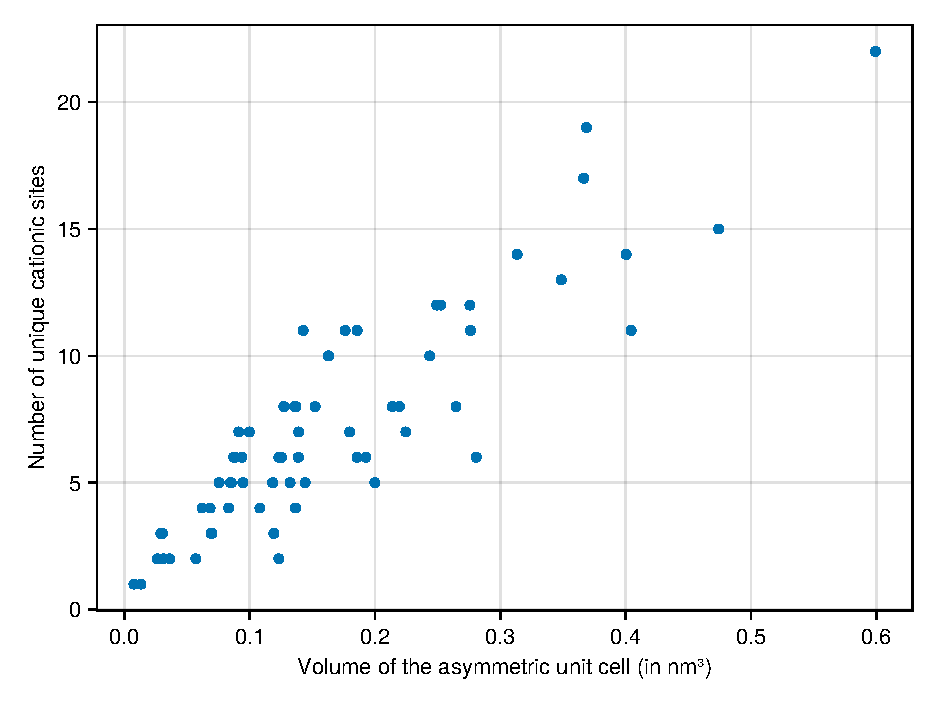
\includegraphics[width=0.65\linewidth]{figures/cations/sitesasymmetricvolumecell.pdf}
	\caption{Correlation between the volume of the asymmetric unit and the number of unique site per zeolite. Coefficient of determination: $R^2 = \num{0.848}$}\label{fig:sitesvolumecell}
\end{figure}

Nonetheless, like for the case of FAU, the repartition of the cations across these sites is far from uniform, making the less populated sites less relevant for analysis. For example, the ANO topology whose site population is represented on \cref{fig:ANO} has 12 identified sites, of which 4 are never populated by more than one cation across all \SiAl ratios.

For this topology, the raw ``shooting star'' results are quite close to those obtained from the refined site hopping methodology augmented with simulated annealing, using the same conditions as in \cref{sitehopping_simulatedannealing}. Similar to the results for FAU represented on \cref{fig:sitehopping_jeffroyFF}, the trends are very similar, but the exact site occupancies sometimes differ, in particular here for site ``\_5''. Once again, this highlights the added value of site hopping simulations in order to obtain precise site population results.

\Cref{fig:ANO_sites8} shows the result of site hopping (still with simulated annealing) on ANO, but using only the 8 most occupied unique sites. With all their symmetric images, these account for 576 site positions per cell (using a $3\times3\times1$ supercell), compared to 828 positions when taking into account all 12 unique sites. These results are almost identical to those represented on \cref{fig:ANO_sites12} for all 12 sites. The influence of possibly spurious sites is thus negligible for the overall repartition of cations with this methodology, which indicates its robustness.

\begin{figure}
	\centering
	\begin{subfigure}{0.95\linewidth}
		\centering
		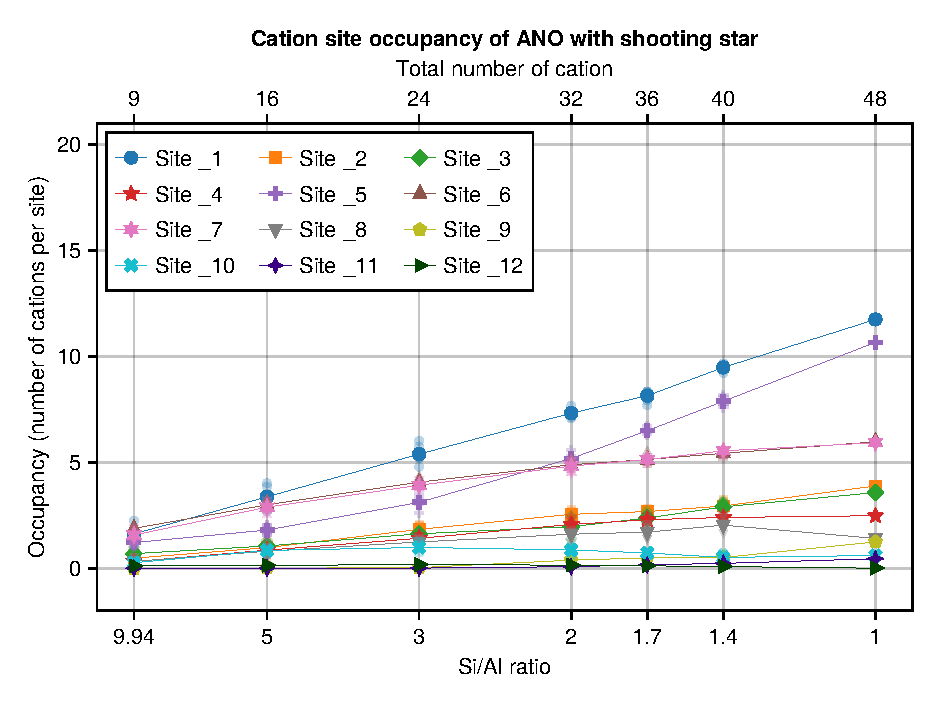
\includegraphics[width=\linewidth]{figures/cations/ANO.pdf}
		\subcaption{Results directly from ``shooting star'' simulations}
	\end{subfigure}

	\begin{subfigure}{0.95\linewidth}
		\centering
		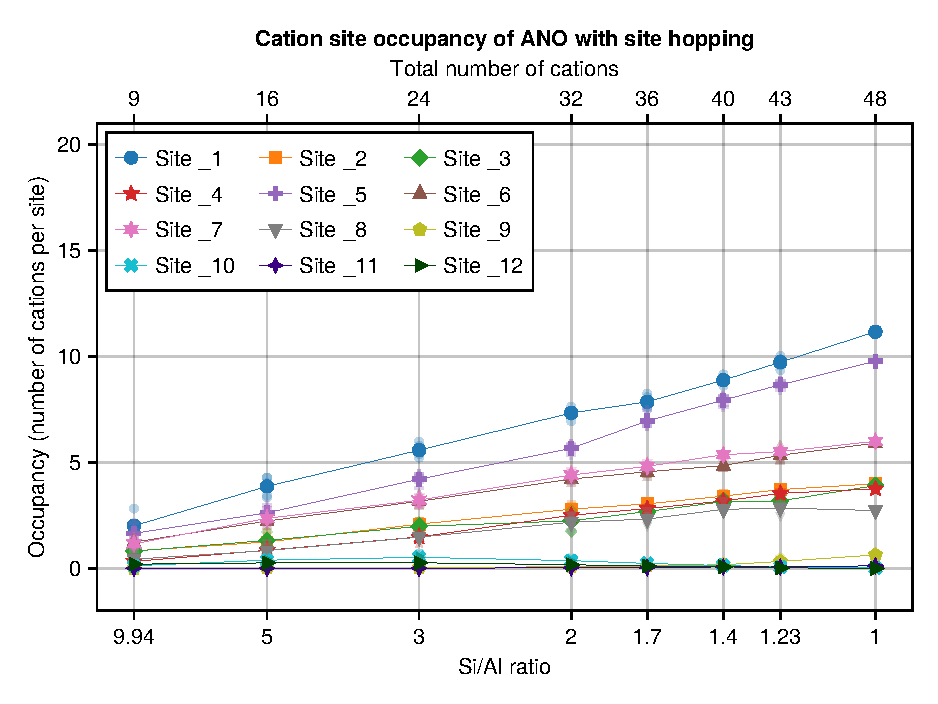
\includegraphics[width=\linewidth]{figures/cations/ANO_sitehopping.pdf}
		\subcaption{Refined results from site hopping with simulated annealing}\label{fig:ANO_sites12}
	\end{subfigure}

	\begin{subfigure}{0.95\linewidth}
		\centering
		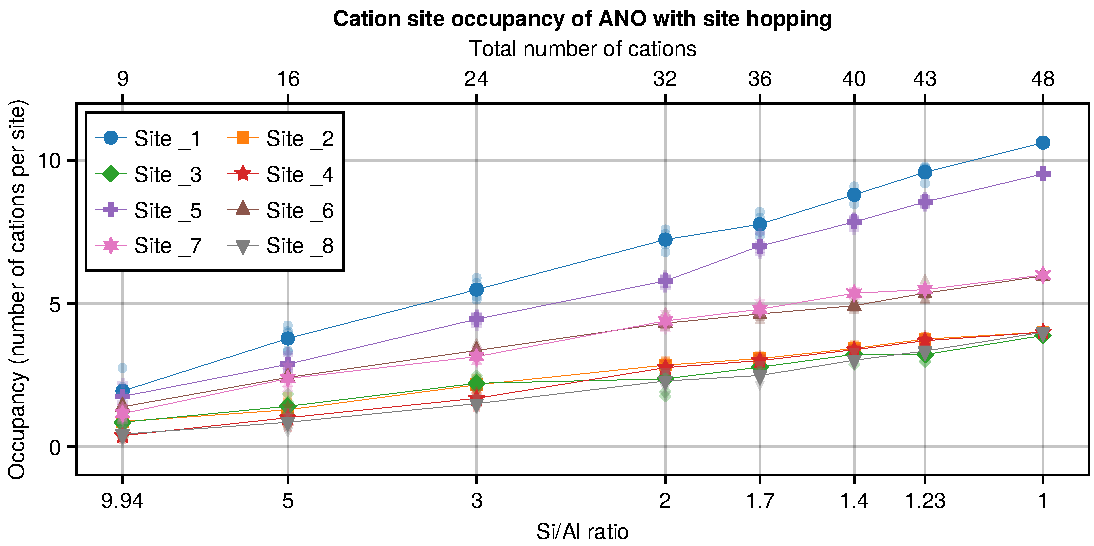
\includegraphics[width=\linewidth]{figures/cations/ANO_sitehopping_sites8.pdf}
		\subcaption{Refined results from site hopping with simulated annealing on only the first 8 sites}\label{fig:ANO_sites8}
	\end{subfigure}

	\caption{Population of each site of ANO}\label{fig:ANO}
\end{figure}

Overall, the proposed methodology for identifying the cationic sites of a zeolite consists in running ``shooting star'' simulations of the target topology across different \SiAl ratios, flattening the cation density maps resulting from all the different cold simulations into a single map, from which the location of the sites are extracted. Their population is then found by running site hopping simulations augmented with simulated annealing. This method shows robust results even for zeolites with many sites, and convergence of the intermediate simulations can be controlled systematically.

\section{Energy computation}\label{energy_computation}

All of the previously exposed methods rely on Monte Carlo steps which may, or may not, be accepted, depending on the difference of energy between the two configurations. By far, the greatest computational cost of any of these methods lies in these energy computations; it is therefore crucial to be able to compute it efficiently.

\subsubsection{The RASPA2 software}

RASPA2 is an open-source software developed by \textcite{RASPA} for classical simulations of molecular systems. Although general purpose, it is mainly used with nanoporous materials and in particular for the study of adsorption and diffusion within. RASPA2 implements Monte Carlo schemes with the Metropolis-Hastings algorithm to perform canonical simulations, but also grand canonical for adsorption (see \cref{adsorption}), as well as parallel tempering. Furthermore, it includes Gibbs ensemble simulation, flexible guest species and frameworks, and many other functionalities which were not needed here.

RASPA2 is written in C, a low-level programming language which allows reaching optimal performance, but is tedious to program in. It cannot be used on GPU and is single-threaded. In order to develop new simulation strategies in an easier setting, I re-implemented the algorithms used for both canonical and grand-canonical simulation of rigid species in rigid frameworks using the Julia programming language\autocite{Julia,JuliaDesign}.

The energy computation algorithms detailed herein are those which were implemented in this new code, but most of them follow that implemented in RASPA2. Moreover, RASPA2 was used to validate the new code, by checking that the simulations yielded the correct physical values (energies, adsorption capacities, and such). By contrast, the ``shooting star'' methodology presented before does not exist in RASPA2.

\subsection{Force fields}

\label{forcefields}

The energy of a molecular structure results from the interaction of its constituent atoms, which are intrinsically quantum. At the molecular level, a popular method used is the quantum Density Functional Theory (DFT), which includes a variety of particular methods, each presenting its own compromise between precision and performance. Some alternatives include methods derived from molecular orbital theory. The number of energy computations for a single molecular simulation can be of the order of \qty{10000} however, which would be much too costly with such methods.

What is commonly used instead are classical force fields, which approximate quantum interactions as a sum of classical interactions between each pair of atoms. These pairwise interactions are defined by one formula per pair of nature of atoms; in the case of non-bonded atoms, each formula is simply a function of the distance between the two atoms. Zeolites are mostly rigid materials, which means that their deformation due to their vibration modes, or subsequent to the organization of cations or adsorbed gas inside, is negligible for the purpose of the molecular simulation. As a consequence, the interactions between framework atoms can be skipped, the only ones to consider for cation placement are those between the cation and the different atoms of the zeolites, which are not bonded.

The pairwise interaction formula is usually divided between the energy contribution of the charges of the atoms, and a short-range van der Waals term. Designing a force fields thus customarily consists in choosing the atomic charges and the formula for the van der Waals term. Several options have been used in the literature for the latter: a very common option is the Lennard-Jones potential
\[r\mapsto 4\varepsilon\paren{\paren{\frac \sigma r}^{12} - \paren{\frac \sigma r}^6}\label{eq:LJ}\]
where $r$ is the distance between atoms. One alternative is the Buckingham potential
\[r\mapsto A\exp\paren{-B\times r} - \frac C{r^6}\label{eq:Buckingham}\]
The potential parameter $\varepsilon$, $\sigma$, $A$, $B$ or $C$ are part of the design of the force field.

\subsection{Short-term interactions}

Since the van der Waals term decays quickly towards zero, it is computationnally useful to set it to exactly zero beyond a cutoff distance. To do so while avoiding the introduction of unphysical forces, one possibility consists in shifting the formula by a constant, so that the function remains continuous at the cutoff. If no force is required, such as in the MC methods, it is possible to leave the potential unshifted and discontinuous at the cutoff; a tail correction is then added to the total energy to account for the missing interactions (this will be detailed in \cref{tailcorrection}). In any case, knowing that the interaction becomes zero after the cutoff allows some computational optimizations, such as using cell lists in order to iterate over the relevant atom pairs only, instead of all atom pairs.

For simplicity of the implementation, the dimensions of the simulated unit cell must be taken so that for any atoms $A$ and $B$, there is at most one periodic image of $B$ which is lower than the cutoff distance from atom $A$. This translates to the constraint that the orthogonal lengths of the unit cell must be as long as at least twice the cutoff. We take this cutoff as \qty{12}{\angstrom}, as is common in the literature and is the default in RASPA2.

Given this constraint, the total energy of a configuration due to the van der Waals interaction can be computed by summing the contribution of each the pair of atoms which are closer than the cutoff distance. This can done naively with a double loop over all atoms, computing the distance of each pair and rejecting that above the threshold. Here, the distance considered is the periodic distance, \textit{i.e.} the smallest distance between periodic images of the two atoms, respective to the periodicity of the crystal. Computing it is up to 6 times more costly than without periodicity, and can become a computational bottleneck for simple enough force fields.

To avoid unecessary distance computations, a possibility consists in binning the space of the unit cell, and skipping the pairs of atoms that belong to bins further than the cutoff distance. This idea underlies the principle of neighbour list which can be used to obtain the list of relevant pairs of atoms efficiently. We use the CellListMap.jl [10.1016/j.cpc.2022.108452] julia package for this purpose, although we only enable it when the cell is large enough. Indeed, the naive approach can actually be more efficient in many cases where the orthogonal lengths of the cell are close to twice the cutoff distance.

\subsection{Ewald summation}

\subsubsection{Energy decomposition}

In opposition to the van der Waals term, charge interactions do not have a cutoff, because Coulomb's law does not decay fast enough towards zero. The interaction between atoms $A$ and $B$, of respective charge $q_A$ and $q_B$, is:
\[E^\text{Coulomb}_{A,B} = \frac{q_A q_B}{4\pi\varepsilon_0\times \norm{\boldsymbol r_B - \boldsymbol r_A}} = \frac{q_n q_m}{4\pi\varepsilon_0\times \norm{\boldsymbol r_m - \boldsymbol r_n + \boldsymbol l}}\]
where $n$ and $m$ are the unique atom numbers in a reference unit cell of respectively $A$ and $B$, and $\boldsymbol l$ is the lattice vector between the origin of the unit cell of $A$ and that of $B$.
Therefore the total contribution of charge interactions in a crystal with $N$ atoms per unit cell is:
\[E^\text{Coulomb} = \frac12\sum_{A\neq B}E^\text{Coulomb}_{A,B}
                   = \frac1{8\pi\varepsilon_0}\sum_{\boldsymbol l}\underset{n\neq m\text{ if }\boldsymbol l = 0}{\sum_{n=1}^N\sum_{m=1}^N} \frac{q_n q_m}{\norm{\boldsymbol r_n - \boldsymbol r_m + \boldsymbol l}}\]
where $\boldsymbol l$ iterates over the lattice vectors.

The semi-convergence of the sum over $\boldsymbol l$ makes it impossible to compute directly. Hence, several methods have been developped to obtain the result such as particle mesh Ewald (PME) and particle-particle-particle-mesh (P$^3$M). We focus on the initial Ewald summation technique underlying them, which is used in RASPA2 and which we also implemented.

Since the crystal is a periodic system, any function of the system that depends on a position in space can be decomposed into a simple sum by Fourier transform. This is in particular true of the electric potential, hence the problematic sum above could be computed in Fourier space. However, the charges are located on the atoms, and are thus discrete, which causes singularities that prevent the computation. The idea behind Ewald summation consists in fictitiously smoothing the point charges into Gaussians: these smooth charges yield a potential computable in Fourier space, while the potential resulting from the real point charge minus their Gaussian counterpart is computed in real space. Electric potential is additive, so the total electric potential $\Phi(\boldsymbol r)$ is then obtained by adding the real space term $\Phi^\text{direct}(\boldsymbol r)$ and the Fourier term $\Phi^\text{reciprocal}(\boldsymbol r)$. Finally, the resulting energy is simply the action of the point charges on the potential:
\[E^\text{Coulomb} = \frac12\sum_{n=1}^N q_n\paren{\Phi^\text{direct}(\boldsymbol r_n) + \Phi^\text{reciprocal}(\boldsymbol r_n)} - E^{\text{self}}\]
$E^{\text{self}}$ designates a spurious self-interaction energy term which must be substracted.

\subsubsection{Direct term}

To each atom $A$ of the crystal is associated a Gaussian charge density
\[\boldsymbol r\mapsto q_A\paren{\frac\alpha{\sqrt\pi}}^3\exp\paren{-\alpha^2\norm{\boldsymbol r_A - \boldsymbol r}^2}\label{gaussian_charge}\]
Thus, the direct term is the potential resulting from the point charge minus this Gaussian. This can be obtained by solving Poisson's law:
\[-\nabla\Phi(\boldsymbol r) = 4\pi\rho(\boldsymbol r)\label{Poisson}\]
which yields, after some simplification steps not detailed here:
\[\Phi^\text{direct}_A(r) = q_A\frac{\text{erfc}(\alpha r)}r\]
where $r$ is the distance to atom $A$ and $\text{erfc}$ is the complementary error function $\text{erfc} = 1 - \text{erf}$, with $\text{erf}:x\mapsto\frac2{\sqrt\pi}\int_0^xe^{-t^2}\text dt$. Since $\text{erfc}$ quickly decays towards $0$, the total direct potential at a given point can be computed by only considering the contribution of the closest charges around, so
\[\Phi^\text{direct}(\boldsymbol r) \approx \sum_{n=1}^N \frac{q_n}{\pnorm{\boldsymbol r - \boldsymbol r_n}}\paren{\text{erfc}\paren{\alpha \pnorm{\boldsymbol r - \boldsymbol r_n}}}\]
where $\pnorm{\boldsymbol x}$ designates the distance to the origin of the closest periodic image of $\boldsymbol x$.

\subsubsection{Reciprocal term}

For the reciprocal term, we start by writing the total charge density coming from the Gaussians given in \cref{gaussian_charge}:
\[\rho^\text{reciprocal}(\boldsymbol r) = \sum_{\boldsymbol l}\sum_{n=1}^N \frac{q_n}{4\pi\varepsilon_0}\paren{\frac\alpha{\sqrt\pi}}^3\exp\paren{-\alpha^2\norm{\boldsymbol r_n + \boldsymbol l - \boldsymbol r}^2}\]
Its Fourier decomposition over the periodic unit cell of volume $V$ is:
\[\begin{split}
\hat\rho^\text{reciprocal}(\boldsymbol k) &= \frac1V\int_V e^{-i\boldsymbol k\cdot\boldsymbol r} \rho^\text{reciprocal}(\boldsymbol r)\text d\boldsymbol r
\\&= \frac1V\int_\Omega e^{-i\boldsymbol k\cdot\boldsymbol r} \sum_{n=1}^N \frac{q_n}{4\pi\varepsilon_0} \paren{\frac\alpha{\sqrt\pi}}^3\exp\paren{-\alpha^2\norm{\boldsymbol r_n + \boldsymbol r}^2} \text d\boldsymbol r
\\&= \frac{2\pi\alpha^3}{V\pi^{3/2}} \sum_{n=1}^N \frac{q_n}{4\pi\varepsilon_0} e^{-i\boldsymbol k\cdot\boldsymbol r_n} \int_0^\infty \norm{\boldsymbol{r}'}^2\exp\paren{-\alpha^2 \norm{\boldsymbol{r}'}^2}\int_0^\pi e^{-i\boldsymbol k\cdot\boldsymbol{r}'} \sin(\theta) \text d \theta \text d \boldsymbol{r}'
\\&= \frac1{4\pi\varepsilon_0V}\exp\paren{\frac{-k^2}{4\alpha^2}}\sum_{n=1}^N q_n e^{-i\boldsymbol k\cdot\boldsymbol r_n}\end{split}\]
after several simplification steps not detailed here. Using Poisson's law (\cref{Poisson}), the electric potential due to the Gaussians can then finally be expressed as:
\[\Phi^\text{reciprocal}(\boldsymbol r) = \frac{1}{\varepsilon_0V}\sum_{\boldsymbol k\neq \boldsymbol 0}\sum_{n=1}^N \frac{q_n}{k^2} e^{i\boldsymbol k\cdot\paren{\boldsymbol r - \boldsymbol r_n}}\exp\paren{\frac{-k^2}{4\alpha^2}}\label{eq:reciprocal}\]

The term $\kappa_{\boldsymbol{k}} = \frac1{k^2}\exp\paren{-k^2/(4\alpha^2)}$ decays fast, so the sum over $\boldsymbol{k}\neq\boldsymbol{0}$ is actually computed as a sum over a finite number of values of $\boldsymbol{k}$ close to $\boldsymbol{0}$. These values are chosen so that the remaining sum of $\kappa_{\boldsymbol{k}}$ for any $\boldsymbol{k}$ not retained is below the target precision of the computation.

\subsubsection{Self-interaction term}

The last remaining term is the self-interaction, which must be removed. Its existence comes from the way the reciprocal term is computed: $\Phi^\text{reciprocal}(\boldsymbol r)$ includes the contribution of all charges on point $\boldsymbol r$, but there should not be any contribution of atom $A$ at position $\boldsymbol r_A$.

Moreover, in the case of rigid polyatomic molecules, like the small gases we will discuss in \cref{adsorption}, there should not be any contribution of atom $A$ at the positions $\boldsymbol r_B$ of other atoms $B$ part of the same molecule.

Each atom $1\le n\le N$ thus contributes a spurious potential term:
\[\Phi^\text{self}_n = \frac{2\alpha q_n}{\sqrt\pi} + \frac12\sum_{\substack{m\\m\smile n,\ m\neq n}}\frac{q_m\text{erf}\paren{\pnorm{\boldsymbol r_n - \boldsymbol r_m}}}{4\pi\varepsilon_0\pnorm{\boldsymbol r_n - \boldsymbol r_m}}\]
where $m\smile n$ is true when both atoms $m$ and $n$ belong to the same molecule.

\subsubsection{Total charge energy}

Combining the last three terms, we obtain the overall Coulomb energy:
\[\begin{split}
E^\text{Coulomb} &= \sum_{\boldsymbol l} \sum_{n=1}^N\sum_{\substack{m=1\\m\not\smile n}}^n \frac{q_n q_m}{8\pi\varepsilon_0}\frac{\text{erfc}\paren{\alpha\norm{\boldsymbol r_n - \boldsymbol r_m + \boldsymbol l}}}{\norm{\boldsymbol r_n - \boldsymbol r_m + \boldsymbol l}}
\\&+ \frac1{2\varepsilon_0V} \sum_{\boldsymbol{k}\neq\boldsymbol{0}}\sum_{n=1}^N\sum_{m=1}^N \frac{q_n q_m}{k^2}e^{i\boldsymbol k\cdot\paren{\boldsymbol r_m - \boldsymbol r_n}}\exp\paren{\frac{-k^2}{4\alpha^2}}
\\&- \xcancel{\sum_{n=1}^N\frac{2\alpha q_n}{\sqrt\pi}}
- \frac12\sum_{n=1}^N\sum_{\substack{m=1\\m\smile n,\ m\neq n}}^N \frac{q_n q_m}{4\pi\varepsilon_0}\frac{\text{erf}\paren{\pnorm{\boldsymbol r_n - \boldsymbol r_m}}}{\pnorm{\boldsymbol r_n - \boldsymbol r_m}}
\label{eq:totalcoulombenergy}\end{split}\]

The term summing the $2\alpha q_n/\sqrt\pi$ cancels out because the overall system needs to be electrically neutral to carry a physical meaning, so the sum of all $q_n$ is 0. This invariant is checked in the code to avoid any error.

\subsection{Precomputation}

\label{precomputations}

Different algorithms that solve a particular problem generally differ in the specific space-time tradeoff they choose. Obtaining the energy of a configuration presents the same possibility: while entirely computing the energy from scratch requires a set amount of computation, it is possible to make subsequent computations faster at the cost of a greater memory footprint of the algorithm, by storing some intermediate results which can be reused afterwards.

\subsubsection{Energy grid}

\label{energygrid}

In the case of simulations involving a rigid framework, the most obvious precomputation that can be done is that of the short-term interactions of the guest species with the framework atoms. Indeed, such interactions only depend on the nature and the position of the guest atom, so it is possible to store them on an energy grid.

More precisely, fore each possible guest atom, the unit cell of the framework is divided into a regular grid, with a set spacing between consecutive points. We use \qty{0.15}{\angstrom}, which is fine enough to be accurate but not too fine to avoid using too much memory. For each grid point, the sum of the interactions of all framework atoms with a guest atom in that position is stored at that point. The grid is then written to disk.

During the simulation, in order to compute the short-term interactions between the framework atoms and a guest atom at a given position, the value is interpolated from the surrounding grid points. Using a simple linear interpolation of the values does not yield very satisfactory results however, since derivative discontinuity would push that atoms towards the grid points, which would result in simulation artifacts. To prevent this, RASPA2 stores not only the value of the energy, but also the three first derivatives, three values of the second derivatives and one of the third, following a scheme by \textcite{TricubicGridInterpolaction}. Moveover, the grid is forced to be orthorombic: this means that it may not be aligned with the unit cell of the framework, but it does not matter as long as each point in the unit cell can be surrounded by recorded grid points. I reimplemented the same grid algorithm, which ensures a smooth interpolation everywhere in space.

\subsubsection{Ewald precomputation}

Short-term interactions that can be stored in grids include the short-term direct part of the Ewald summation. The reciprocal term cannot however be simply stored as such.

Yet, it is still possible to precompute a large part of the reciprocal interaction which is due to the framework. To take the potential given by \cref{eq:reciprocal} back to the energy, it is useful to introduce the sums:
\[S_{\boldsymbol k} = \sum_{n=1}^N q_n e^{-i\boldsymbol k\cdot \boldsymbol r_n}\label{eq:Sk}\]
for each $\boldsymbol k$. With this notation, the contribution of the reciprocal term to the energy is
\[\begin{split}
E^\text{reciprocal} &= \frac12\sum_{m=1}^N q_m \Phi^\text{reciprocal}(\boldsymbol{r}_m)
\\&= \frac1{2\varepsilon_0V} \sum_{m=1}^N q_m \sum_{\boldsymbol{k}} \kappa_{\boldsymbol k} e^{i\boldsymbol k\cdot\boldsymbol r_m}S_{\boldsymbol{k}} \quad\text{ then using }\overline{S_{\boldsymbol{k}}} = \sum_{m=1}^N q_me^{i\boldsymbol k\cdot\boldsymbol r_m}
\\&= \frac1{2\varepsilon_0V} \sum_{\boldsymbol{k}} \kappa_{\boldsymbol k} \overline{S_{\boldsymbol{k}}} \times S_{\boldsymbol{k}}
= \frac1{\varepsilon_0V} \sum_{\boldsymbol{k}} \kappa_{\boldsymbol k} \norm{S_{\boldsymbol{k}}}^2
\end{split}\]

Hence, to avoid redundant computations, the list of relevant $\boldsymbol{k}$, associated to their factor $\kappa_{\boldsymbol k} = \exp\paren{-k^2/\paren{4\alpha^2}}/k^2$, is computed once and for all. For each atom $n$ of the framework, the factors $q_n\exp\paren{i\boldsymbol{k}\cdot\boldsymbol{r}_n}$ are also computed once.
Distinguishing between the atoms of the framework and the guests allow separating $S_{\boldsymbol k}$ into $S_{\boldsymbol k}^\text{framework} + S_{\boldsymbol k}^\text{guest}$, so that finally, the energy can be computed as
\[E^\text{reciprocal} = \underbrace{
	\frac1{2\varepsilon_0V} \sum_{\boldsymbol k} \kappa_{\boldsymbol k}\norm{S_{\boldsymbol k}^\text{framework}}^2 + \frac1{2\varepsilon_0V} \sum_{\boldsymbol k}\kappa_{\boldsymbol k} \left(\overline{S_{\boldsymbol k}^\text{framework}}\right.
}_\text{precomputed part}
+ \left.\overline{S_{\boldsymbol k}^\text{guest}}\right) \times S_{\boldsymbol k}^\text{guest}\label{eq:reciprocal_decomposed}\]

%Hence, \cref{eq:reciprocal} can be rewritten as
%\[\begin{split}\Phi^\text{reciprocal}(\boldsymbol r) &= \frac{1}{\varepsilon_0V}\sum_{\boldsymbol k\neq \boldsymbol 0}e^{i\boldsymbol{k}\cdot\boldsymbol{r}}\underbrace{\frac1{k^2}\exp\paren{\frac{-k^2}{4\alpha^2}}\left(\sum_{n\text{ framework}} q_n e^{-i\boldsymbol k\cdot\boldsymbol r_n}\right.}_\text{precomputed part}\left. + \sum_{n\text{ guest}} q_n e^{-i\boldsymbol k\cdot\boldsymbol r_n}\right)
%\\&= \frac1{\varepsilon_0V}\sum_{\boldsymbol k\neq \boldsymbol 0} \kappa_{\boldsymbol k} F_{\boldsymbol k} e^{i\boldsymbol{k}\cdot\boldsymbol{r}} \ +\  \frac1{\varepsilon_0V}\sum_{\boldsymbol k\neq \boldsymbol 0} \kappa_{\boldsymbol k} e^{i\boldsymbol{k}\cdot\boldsymbol{r}} \sum_{n\text{ guest}} q_n e^{-i\boldsymbol k\cdot\boldsymbol r_n}
%\label{eq:reciprocal_decomposed}\end{split}\]
%where $\kappa_{\boldsymbol k} = \frac1{k^2}\exp\paren{-k^2/(4\alpha^2)}$ and $F_{\boldsymbol k} = \sum\limits_{n\text{ framework}} q_n e^{-i\boldsymbol k\cdot\boldsymbol r_n}$ are precomputed terms.

Finally, the entire self-interaction term can be computed once for all, since it does not depend on the configuration. This is only the case here because the simulated moleculses are rigid bodies; for deformable structures, the self-interaction term depends on the actual conformation of the guests, which may depend on the state.

\subsubsection{Optimizations for computing the difference of energies}

\label{energydifference}

A simulation that follows the Metropolis-Hastings algorithm walks across configurations, each pair of contiguous states being separated by a single MC move. In this context, computing the energy of each trial configuration to compare it to the previous one is wasteful: the only part of the energy impacted by the MC move is that which stems from the moved species. Instead of computing the energy of the trial configuration, it is thus better to directly compute the energy difference due to the move.

For the short-term interactions, this is straightforward: the energy difference is simply the sum of the interactions of the species at the new position minus that at its previous position. If there are $N$ species, moving one thus costs $O(N)$ computations for these terms, instead of $O(N^2)$ required to compute this energy the first time. The direct part of the Ewald summation follows the same principle.

For the reciprocal part, the difference in energy is derived from \cref{eq:reciprocal_decomposed} by removing the first constant term and computing:
\[\Delta E^\text{reciprocal} = \frac1{2\varepsilon_0V} \sum_{\boldsymbol k}\kappa_{\boldsymbol k} \left(
\overline{S_{\boldsymbol k}^\text{framework}}\times\Delta S_{\boldsymbol k}^\text{guest} +
\Delta \norm{S_{\boldsymbol k}^\text{guest}}^2
\right)\label{eq:reciprocal_move}\]
%\[\Delta_\text{move}\Phi^\text{reciprocal}(\boldsymbol{r}) = \frac1{\varepsilon_0V}\sum_{\boldsymbol{k}\neq\boldsymbol{0}} \kappa_{\boldsymbol k}e^{i\boldsymbol k\cdot\boldsymbol{r}} \sum_{n\text{ moved}}q_n\paren{e^{-i\boldsymbol k\cdot\boldsymbol{r}'_n} - e^{-i\boldsymbol k\cdot\boldsymbol r_n}}\]
Since both values of $S_{\boldsymbol k}^\text{guest}$ need to be computed before and after the move to take the difference of their norm, it is actually equally efficient to directly compute both values of $E^\text{reciprocal}$ before and after the move, directly following \cref{eq:reciprocal_decomposed}, and taking the difference, instead of the previous formulation.

In order to allow computing this efficiently, each term $q_ne^{-i\boldsymbol k\cdot\boldsymbol r_n}$ is thus stored in memory (instead of recomputing it each time). The new values $q_ne^{-i\boldsymbol k\cdot\boldsymbol{r}'_n}$ computed for the trial move are also temporarily kept in memory, so they can be used to replace the previous ones if the trial move is accepted. Finally, the value of each $S_{\boldsymbol{k}}^\text{guest}$ is also kept in memory, so that it can be updated by reusing the previous computation.

RASPA2 does not implement this optimization, and simply recomputes the $e^{-i\boldsymbol k\cdot\boldsymbol r_n}$ terms each time, which is slower but requires less memory.

\subsubsection{Blocking pockets}
\label{blockingpockets}

Some MC trial moves attempt to displace an atom to a location that would lead to unphysically high energies -- typically, too close to a framework atom. Such positions can be determined once and for all, and the relevant MC moves automatically rejected without the need for any energy computation.

The simplest strategy to do so consists in making a boolean grid, aligned with the energy grids used for short-term interactions, which stores a 1 when the voxel is blocked or 0 if it is allowed. The first step of any MC trial move then consists in checking whether each atom is in an allowed voxel, or rejecting the move otherwise. In practice, the simplest implementation consists in making one such boolean grid per atom kind (since the value of the framework-atom interaction energy depends on the atom), and for each actual atom position, checking the closest grid point of its kind.

In addition to its use as computational optimization, such boolean grids can also be used to mark some parts of the framework as inaccessible, irrespective of the corresponding energy. This is useful when small window size prevents a species -- for instance a gas molecule -- from entering a pore -- for instance the sodalite cages in LTA zeolites [10.1021/ja953856q]. Indeed, without explicitly blocking the pocket, an MC move could make a species appear in the pore, whereas it should be kinetically impossible to enter. This strategy will thus be used when studying the adsorption of gases in zeolites (see \cref{adsorption}), but for the small cations under study here, there is no need to additionally block any part of the frameworks.

RASPA2 only implements blocking for the latter case -- \textit{i.e.} explicit pocket removal. It does not use a boolean grid: instead, the blocked space is described as a combination of blocking spheres. For each trial move, the distance between the atoms of the moved guest and the center of each sphere is computed: if one is below its radius, the move is rejected. This approach requires less precomputation and thus less memory than storing the boolean grids, but its runtime cost is much greater, and increases with the number of blocking spheres, preventing it from being used as an optimization like before. It is thus less efficient than the approach I implemented.

These boolean grids are also useful to improve the acceptance rate of reinsertions. When a reinsertion move is attempted, a new position for the species is chosen at random in the unit cell, but it is then immediately checked against the blocking pocket grids. If the attempted position is forbidden, a new random position is chosen, and so iteratively until finding a position compatible with the boolean grid constraints. This trial position is then used as any other trial moves, and can be accepted or rejected based on the energy criterion. Crucially, biasing the choice of the reinsertion trial move in this fashion improves its acceptance rate while still maintaining the detailed balance of the simulation, because a reinserted species was necessarily located in a position that was not blocked by the boolean grids either. Note that this bias cannot be used for local translations or rotation however: if a trial translation moves a species in a blocked pocket, the move must be rejected.

\subsubsection{Site hopping precomputations}

The main computational advantage of site hopping simulations, defined in \cref{sitehopping}, is that the number of sites is fixed in advance, which allows precomputing all framework-site and site-site interactions.

To do so, the value of the framework-site interaction energy is computed and stored for each site by computing the energy associated with putting only one cation in the framework at the position of the site. However, this energy is actually ill-defined, since placing only one cation in the framework means that the unit cell has a net charge, and thus the (infinite periodic) material has an infinite charge. Moreover, even disregarding the physical absurdity of this scenario, a net charge would lead to a non-zero $\sum_{n=1}^N2\alpha q_n/\sqrt\pi$ term, even though it was removed in \cref{eq:totalcoulombenergy}. Still, the computations can be carried to yield a numerical value, which is thus stored in a list $\text{framework}[i]$ where $i$ designates the index of a particular site $s_i$. The reciprocal ewald contribution of this energy is also temporarily stored in a separate list as $r_i$.

Likewise, for each pair $(s_i,s_j)$ of sites, the energy of the framework containing only two cations, one in $s_i$ and one in $s_j$, is computed as $e_{i,j}$, although it also does not carry physical sense either. What is stored in a matrix is
$\text{interaction}[i,j] = e_{i,j} - r_i - r_j$.
This is only possible if the number of sites is not too high, since the number of interactions to store grows quadratically with the number of sites and would become prohibitively high otherwise.

Finally, the tail correction $\text{tc}_n$ associated with the framework filled with $n$ cations is computed once, where $n$ is constrained by the number of aluminiums in the structure.

Using these unphysical values, the actual physical energy of a real configuration with $n$ cations on sites $s_{k_1}, s_{k_2}, \ldots, s_{k_n}$ can then be computed as
\[E(s_{k_1}, s_{k_2}, \ldots, s_{k_n}) = \text{tc}_n + \sum_{i=1}^n\text{framework}[k_i] + \sum_{1\le i<j \le n}\text{interaction}[k_i,k_j]\]
and the energy associated with a trial move of one cation can thus be computed with only $n$ array reads, which is optimally efficient.

As previously emphasized, the components $\text{framework}[i]$ and $\text{interaction}[i,j]$ should not be considered individually to assess the stability of a particular site. Indeed, $\text{framework}[i] < \text{framework}[j]$ does not necessarily mean that site $s_i$ is more populated than $s_j$, because the site-site interaction energies could make the total energy $E$ systematically higher when $s_i$ is populated rather than $s_j$, which is the true measure of a site stability.

\section{Possible alternatives}

\label{metadynamics}

Molecular dynamics (MD) could also be used to place cations in zeolites. Generally speaking, the principle of MD consists in running a simulation where the particles follow Newton's laws of motion, with forces based on force fields like for MC schemes. The simulation is divided in time steps, between which the forces are computed on each particle to derive their position at the next time step. Hence, the trajectories of the particles in MD follow a physical path.

Temperature can be included in different ways in MD, all of which use an element of randomness that eventually impacts the velocities of particles, in order to ensure that the average values extracted from the simulation correspond to those which would be obtained at that temperature. This means that the precedent discussion on the inaccessibility of high-energy regions to the system at room temperature still applies in MD.\@ A simple MD simulation is thus doomed to only explore local energy minima, failing to reach ergodicity like with the simple canonical MC scheme.

To circumvent this issue, it is necessary to bias the simulation in order to force the system to explore regions of high energy. One such strategy consists in doing metadynamics\autocite{Metadynamics}, which is a variation of MD in which the potential energy landscapes is modified during the simulation. The effective free energy of a point in configuration space is computed as the sum of the real free energy of that point without bias, added to the sum of some Gaussian functions centred on previously explored points. Every few steps, another Gaussian function centred on the current configuration point is added to the bias, so that the effective free energy of explored regions increases through the simulation, which allows the system to eventually escape local minima and explore other regions.

A Gaussian is a function of the form $f:\boldsymbol x\mapsto Ae^{-\paren{\boldsymbol x - \boldsymbol\mu}^\top\Sigma\paren{\boldsymbol x - \boldsymbol\mu}}$. In practice, the variable $\boldsymbol x$ of the Gaussians used in metadynamics are not directly the $3N$ coordinates of the $N$ particles, but a small-dimensional vector whose coordinates are called ``collective variables''. These collective variables are themselves function of the $3N$ initial coordinates. The parameter $A$ and $\Sigma$ of the Gaussians being usually fixed, each Gaussian is stored by its centre $\boldsymbol\mu$, whose coordinates are thus the collective variables of the current configuration point. Therefore, compared to regular MD, running a metadynamics simulation incurs the additional cost of computing the collective variables $\boldsymbol x$ of each visited configuration point, storing the Gaussians' centres, and computing their value at each step.

For cation placement the main issue is to find a small set of relevant collective variables, since the cost of metadynamics grows with their number. We did not explore this venue because we expected it to be similar in difficulty to the MC alternatives, with no clear reason why it should be more efficient. MD in general is also known to converge more slowly than MC, because large configuration change made possible by MC steps are prohibited by the physics-driven approach of MD, and the same argument could be made of metadynamics compared to other accelerated MC schemes. Exploring metadynamics or its variants could nonetheless be of interest in the search for more alternative, and potentially more efficient, algorithms.

\OnlyInSubfile{\printglobalbibliography}

\end{document}
